\documentclass[12pt,a4paper]{report}

\usepackage[backend=biber, style=ieee]{biblatex}
\addbibresource{literature.bib}

\usepackage{lmodern}
\usepackage{microtype}
\usepackage{parskip}
\usepackage{float}
\usepackage{enumitem}
\usepackage{tabularx}
\usepackage{graphicx}

\usepackage[utf8]{inputenc}
\usepackage[T1]{fontenc}
\usepackage[ngerman]{babel}
\usepackage[onehalfspacing]{setspace}

% Präambel:
\usepackage{tikz}
\usetikzlibrary{arrows.meta,positioning}
\tikzset{
  step/.style = {rectangle, rounded corners, draw, align=center,
                 minimum width=6.5cm, minimum height=7mm, fill=gray!5},
  ->/.style = {-{Latex[length=2mm,width=2mm]}}
}


\usepackage{xcolor}
\newcommand{\todo}[1]{\colorbox{red}{\textbf{TODO: #1}}\\}
\newcommand{\question}[1]{\colorbox{yellow}{\textbf{QUESTION: #1}}\\}
\newcommand{\xeno}[1]{\colorbox{pink}{\textbf{TODO XENO: #1}}\\}
\newcommand{\gideon}[1]{\colorbox{green}{\textbf{TODO GIDEON: #1}}\\}

\begin{document}

\begin{titlepage}
  \centering
  {\huge \textbf{Plattform zur Analyse von Entwicklerzufriedenheit und Produktivität in agilen Teams} \par}
  {\large IP5 Projekt \par}
  \vspace{0.5cm}
  {Windisch, August 2025 \par}
  \vspace{0.5cm}

  \begin{figure}[H]
    \centering
    
\includegraphics[width=0.60\textwidth]{../figures/logo.png}
  \end{figure}

  \vfill
  \begin{tabular}{@{}ll@{}}
    \textbf{Studenten:}    & Xeno Isenegger, Gideon Monterosa \\
    \textbf{Fachbetreuer:} & Norbert Seyff, Nitish Patkar
  \end{tabular}

  {Fachhochschule Nordwestschweiz, Hochschule für Informatik \par}
\end{titlepage}

\chapter*{Abstract}
\todo{Abstract und Keywords schreiben}
\newpage

\todo{Kapitel klickbar machen}
\todo{überprüfen ob sinnvolle namen und die richtigen titel angezeigt werden}
\tableofcontents
\newpage

\listoffigures
\newpage

\listoftables
\newpage

\chapter{Einleitung}

\section{Motivation}
\todo{spellcheck}
\todo{gendern überprüfen}

Die Zufriedenheit von Entwicklerinnen und Entwicklern wird, wenn überhaupt, meist nur anhand der
Menge ihrer geleisteten Arbeit gemessen. Dabei entstehen zwangsläufig Defizite, und ein halbjährli-
ches Mitarbeitergespräch erweist sich oft als wenig wirksame Massnahme zur Problemlösung.

Dieses Projekt baut auf einer bestehenden Arbeit auf, in der eine Plattform zur Erfassung der Ent-
wicklerzufriedenheit entwickelt wurde. Die Webapplikation Yappi ermöglicht es Entwicklerinnen und
Entwicklern, ihre Zufriedenheit mit ihrer Arbeit und ihrer aktuellen Situation fortlaufend zu bewerten.
Yappi erfasst emotionale Faktoren wie Happiness sowie weitere Zufriedenheitsindikatoren. Zusätz-
lich können spezifische Aufgaben und Arbeitstypen individuell bewertet werden. Die erhobenen Da-
ten werden anonym auf Teamebene analysiert, um ein fundiertes Verständnis für die Stimmung in-
nerhalb der Teams zu gewinnen.

Entwicklerinnen und Entwickler haben die Möglichkeit, ihre Zufriedenheit für verschiedene Teams zu
erfassen, wodurch gezielte Analysen ermöglicht werden. Unternehmen erhalten dadurch wertvolle
Einblicke, um das Arbeitsumfeld gezielt zu verbessern.

Dieses Projekt baut auf Yappi auf und zielt darauf ab, die Erfassung der Zufriedenheit weiter zu opti-
mieren. Es wird untersucht, wie die Daten noch präziser erfasst und ausgewertet werden können,
um langfristige Verbesserungen zu unterstützen. Diese Arbeit dient als Grundlage für ein weiterfüh-
rendes Forschungsprojekt, das sich vertieft mit der Entwicklerzufriedenheit auseinandersetzt und
zusätzliche Erkenntnisse gewinnen soll.

\section{Ziele und Vision}
\todo{überarbeiten evt entfernen}

Yappi wird zu einer umfassenden Plattform weiterentwickelt, die nicht nur die Zufriedenheit misst,
sondern sich nahtlos in den Arbeitsalltag integriert und wertvolle Handlungsempfehlungen liefert.
Dazu werden folgende Kernaspekte umgesetzt:

\begin{enumerate}
  \item \textbf{Produktivitätsfaktoren identifizieren}\\
    Durch eine tiefere Analyse von Zufriedenheitsindikatoren sollen zentrale Faktoren ermittelt werden,
    die sich positiv oder negativ auf die Produktivität und das Wohlbefinden von Entwicklerinnen und
    Entwicklern auswirken. Diese Erkenntnisse werden genutzt, um Vorschläge zu Verbesserungsmass-
    nahmen abzuleiten.
  \item \textbf{Integration in den Arbeitsprozess}
    Yappi soll sich direkt in bestehende Arbeitsabläufe einfügen, um die Erfassung der Zufriedenheit
    möglichst intuitiv und effizient zu gestalten. Dies kann durch verschiedene Schnittstellen und Erwei-
    terungen erfolgen, die eine nahtlose Interaktion ermöglichen.
  \item \textbf{Erweiterung um kontextbezogene Daten}
    Um ein umfassenderes Bild der Arbeitszufriedenheit zu erhalten, können weitere Einflussfaktoren
    berücksichtigt werden. Dazu gehören beispielsweise arbeitsbezogene Rahmenbedingungen oder
    individuelle Gesundheits- und Belastungsindikatoren. Diese Daten sollen helfen, ein besseres Ver-
    ständnis für langfristige Trends und Zusammenhänge zu entwickeln.
  \item \textbf{Intelligente Analyse und Handlungsempfehlungen}
    Durch die Integration von AI schnittstellen können gezielte Analysen erstellt und individualisierte
    Empfehlungen abgeleitet werden. Dies kann sowohl auf individueller als auch auf Teamebene erfol-
    gen, um nachhaltige Verbesserungen im Arbeitsumfeld zu fördern.
\end{enumerate}

\subsubsection{Fazit}

Mit diesen Erweiterungen wird Yappi zu einem essenziellen Bestandteil des Entwickleralltags. Es
bietet nicht nur eine präzisere Erfassung der Zufriedenheit, sondern liefert auch wertvolle Einblicke
und Handlungsempfehlungen, um die Arbeitsbedingungen nachhaltig zu verbessern. Unternehmen
erhalten fundierte Analysen und können gezielt Massnahmen ergreifen, um eine motivierte und pro-
duktive Entwicklergemeinschaft zu fördern.

In der Umsetzung dieses Projekts liegt der Schwerpunkt auf den ersten drei genannten Zielen, mit besonderem Fokus auf die
Integration in bestehende Arbeitsprozesse sowie die Erweiterung um kontextbezogene Daten. Die Identifikation von
Produktivitätsfaktoren wird im Rahmen der Datenerhebung und -analyse vorbereitet, um künftig eine fundierte Ableitung von
Verbesserungsvorschlägen zu ermöglichen. Das vierte Ziel, die Entwicklung einer intelligenten Analyse- und Empfehlungskomponente,
wird in diesem Projekt konzeptionell erarbeitet, jedoch noch nicht technisch umgesetzt. Auf diese Weise wird eine solide Grundlage
geschaffen, um zukünftig auch das vierte Ziel zu erreichen. Die Umsetzung dieses Ziels wird in einer folgenden Bachelorarbeit
genauer thematisiert.

\section{Fragestellungen}

\todo{Einleitung wie diese Fragen aus dem Zielbild entsteht und wie diese Fragen in diesem Projekt beantwortet werden}
\todo{Fragen 1-2 werden umgesetzt Frage 3 wird konzeptionell ausgearbeitet evt in beantwortung}

\begin{enumerate}[label=\Alph*.]
  \item Durch welche Technologien und Schnittstellen kann Yappi erweitert werden,
        um ein reibungsloses und einfaches Erfassen von Zufriedenheitsdaten zu ermöglichen?
        \begin{enumerate}[label=\alph*.]
          \item Entwicklung von Entwickler-Tool-Plugins, die nahtlos in bestehende Arbeitsumgebungen
                integriert werden können, um die Nutzung von Yappi angenehmer und effizienter zu gestalten.
                Diese Plugins sollen Entwicklern ermöglichen, direkt in ihrer bevorzugten Umgebung Feedback
                zu erfassen, ohne den Arbeitsfluss zu unterbrechen. Integration von Yappi in verschiedene
                Plattformen und Tools wie Webbrowser, IntelliJ, Microsoft Teams und Outlook.
        \end{enumerate}
  \item Wie können Gesundheitsdaten in die Auswertung der Entwicklerzufriedenheit einfliessen?
        \begin{enumerate}[label=\alph*.]
          \item Direkte Anbindung der Gesundheitsdaten-API, um relevante Gesundheitsmetriken wie
                Herzfrequenz, Schlafqualität oder Stresslevel automatisch in die Analyse der
                Entwicklerzufriedenheit zu integrieren. Dies ermöglicht eine genauere Einschätzung des
                Wohlbefindens und potenzieller Belastungsfaktoren.
        \end{enumerate}
  \item Wie kann Yappi Teams und Entwickler dabei unterstützen, aus den erfassten
        Zufriedenheitsdaten Handlungsempfehlungen abzuleiten, um die Zufriedenheit und Produktivität
        von Entwicklern zu erhöhen?
        \begin{enumerate}[label=\alph*.]
          \item Entwicklung eines Yappi Coach, der anhand einer detaillierten Analyse der erfassten
                Daten gezielte Tipps zur Verbesserung der Arbeitsweise gibt. Beispielsweise könnte der Coach
                darauf hinweisen, dass Meetings nicht länger als 1,5 Stunden dauern sollten, da längere
                Sitzungen die Zufriedenheit und Konzentration der Entwickler negativ beeinflussen können.
          \item Integration von KI-gestützten Diensten, die auf Basis der gesammelten Gesundheitsdaten
                sowie Zufriedenheits- und Produktivitätsmetriken individuelle Massnahmen vorschlagen. Diese
                KI-gestützten Empfehlungen können Teams dabei helfen, gezielt Optimierungen vorzunehmen, um
                die Arbeitsbedingungen und die Effizienz der Entwickler nachhaltig zu verbessern.
        \end{enumerate}
\end{enumerate}

\chapter{Hintergrund}

\todo{kurze Einleitung oder mergen mit methoden und Einleitung}

\section{Ausgangslage}

Yappi ist eine Webplattform zur Erfassung der Entwicklerzufriedenheit und produktionsnaher Kennzahlen. Ziel ist eine regelmässige,
datenbasierte Diskussion im Team und ein besseres Verständnis wiederkehrender Muster der Teamstimmung. Die Vorgängerarbeit
definiert dafür eine klare Produktvision und liefert ein erstes Minimum Viable Product (MVP) als Grundlage. Die Plattform 
fokussiert sich auf Selbst-Reporting zur Auswertung der Entwicklerzufriedenheit. Der Ansatz adressiert typische Schmerzpunkte
agiler Teams und stützt sich auf Interviews, Literatur und abgeleitete Produktziele. Yappi erlaubt die Erfassung von
Happiness-Daten, deren Auswertung im Dashboard und Vergleiche innerhalb eines Teams. Die Lösung ist so ausgelegt, dass in
Retrospektiven datenbasierte Gespräche geführt werden können.

Yappi ist als Open-Source-Projekt veröffentlicht. Die Repositories für Backend, Frontend und Infrastruktur sind getrennt 
organisiert. Eine lauffähige Instanz steht zu beginn dieses Projektes nicht zur verfügung. Die Zielgruppe ist klar beschrieben. 
Angesprochen sind agile Software-Teams, Scrum Master und Product Owner unterschiedlicher Unternehmensgrössen. Die Vorgängerarbeit
hat die methodische Basis gelegt. Sie umfasst Literaturrecherche, Interviews, abgeleitete Problemfelder, User Flows, Produktziele
und die Validierung der Konzeptlösung. Das vorliegende Projekt baut auf dieser Struktur auf und fokussiert nun auf Integration,
Erweiterbarkeit und vertiefte Analytik.

\section{Aktueller technischer Stand}

\begin{figure}[H]
  \centering
  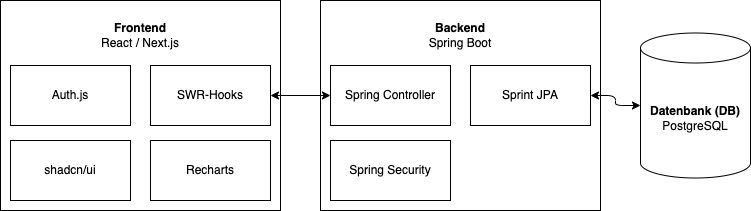
\includegraphics[width=0.95\textwidth]{../figures/before-system-diagram.drawio.png}
  \caption{Systemarchitektur von Yappi vor dem Projekt}
  \label{fig:systemarchitektur}
\end{figure}
\todo{kleiner Text zum Diagram}

\begin{description}
  \item[Backend] Das Backend ist mit Spring Boot umgesetzt. Als Datenbank ist PostgreSQL im Einsatz. Die Kommunikation zum Frontend
    erfolgt über REST-Schnttstellen, welche nach dem OpenAPI standart dokumentiert sind. Die Kommunikation zur Datenbank erfolgt
    über Spring JPA.
  \item[Frontend] Das Frontend basiert auf React und Next.js mit TypeScript. Für Aufrufe werden SWR-Hooks verwendet, dabei handelt
    es sich ume eine React library um Daten zu laden. Komponenten werden mit der Library wird shadcn/ui aufgebaut. Die 
    Visualisierungen entstehen mit Recharts. Um die Codequalität sicherzustellen wird ESLint zur statischen Code analyse und 
    Prettier zur automatischen Formatierung nach vordefinierten Guidelines verwendet.
  \item[Authentisierung und Autorisierung] Die Anmeldung erfolgt über OAuth 2.0. Dabei werden Anbieter wie Google oder GitHub 
    über Auth.js unterstützt. Passwörter werden nicht gepseichert. Die Anfragen ans Backend werden mit JSON Web Tokens (JWT) 
    abgesichert. Die Sicherheitsmechanismen im Backend sind mit Spring Security implementiert.
  \item[Datenmodell] Das relationale Schema umfasst unter anderem Benutzer, Teams, Sprints sowie Umfragetypen für Happiness,
    Emotionen und Work-Kinds.
  \item[Deployment] Die Komponenten sind grösstenteils containerisiert mit Docker. Eine funktionierende CI/CD-Pipeline ist aktuell
    nicht vorhanden. Bestehende Images sind im GitHub Container Registry abgelegt. Für den Betrieb wird eine Linux-VM wie z.B. auf
    der Switch-Engine-Infrastruktur benötigt.
\end{description}
\section{Parallele Entwicklung auf gemeinsamer Codebasis}

\todo{Zusammenarbeit kurz erklären mit Auswirkungen auf unser Projekt}

\section{Stakeholder}

Das Projekt umfasst die folgenden Stakeholder:

\begin{description}
  \item[Primäre Nutzergruppen] Softwareentwickelnde, Scrum Master und Product Owner in agilen Teams. 
  \item[Organisationen] Unternehmen nutzen Yappi, um Kultur und Zusammenarbeit datenbasiert zu verbessern.
  \item[Akademische Stakeholder] Betreuende Dozierende und das Institut an der FHNW welche das Projekt begleiten.
  \item[Betrieb und Entwicklung] Projektteam dieses Projekts und anderer Projekte die auf Yappi aufbauen.
\end{description}

\chapter{Methoden}
\todo{Kanban erwähen}
\section{Projektmethodik}
\section{Prototypen}
\section{Proof of Concepts}
\todo{Abgrenzung bezüglich Datenschutz}
\todo{arc42 erwähen}

\chapter{State of the Art}
\section{Definition von Entwiklerzufriedenheit}

Entwicklerzufriedenheit wird in der Literatur als Balance zwischen positiven und negativen Erlebnissen bei der
Arbeit definiert. Darunter versteht man eine Sequenz von Erfahrungen, bei der häufige positive Emotionen ein
hohes Glücksgefühl erzeugen und häufige negative Erfahrungen das Gegenteil bewirken \cite{sadowski_happiness_2019}.
Auch Industriequellen fassen Entwicklerzufriedenheit als subjektives Wohlbefinden in Bezug auf Arbeitsinhalte
und -umfeld auf, d.h. als Mass für Zufriedenheit, Freude oder innere Zufriedenheit bei der Arbeit \cite{zenhub_2022_nodate}.
Zufriedene Entwickler empfinden demnach mehr Arbeitsfreude und Inhaltlichkeit in ihrer Rolle, was eng mit
der Arbeitsmotivation und dem Engagement bei der Arbeit verknüpft ist \cite{franca_motivation_2020}.

Eng verwendt mit der Zufriedenheit ist der Begriff \textbf{Flow}. In Anlehnung an Csikszentmihalyis Konzept beschreibt
Flow einen Zustand von völliger Vertiefung und hohen Fokus beim Programmieren. Flow tritt dann auf, wenn die Anforderungen
einer Aufgabe im Gleichgewicht mit dem Fähigkeiten des Entwicklers stehen, wodurch man in einen Zustand von intensiver 
Konzentration gelangt. Zufriedene Entwickler gelangen einfacher in einen anhaltenden Flow-Zustand. Unzufriedenheit
hingegen unterbricht diesen Flow, was zu Frustration führt und Schwierigkeiten führt, nach Unterbrechungen wieder in
eine Aufgabe zurückzufinden. Teilnehmer einer Untersuchung berichten, negative Erlebnisse reissen einen aus dem Flow
Zustand und machen es schwer, die Arbeit wieder aufzunehmen \cite{sadowski_happiness_2019}.

Motivation und Zufriedenheit hängen eng zusammen, sind aber konzeptionell unterscheidbar. Motivierte Entwickler sind
zeigen hohes Engagement und Fokus auf ihre Aufgaben, während Zufriedenheiteher durch allgemeines Wohlbefinden und gute
Laune charakerisiert ist. Faktoren wie Autonomie, Kompetenzerleben und Zugehörigkeitsgefühl steigern die intrinsische 
Motivation von Entwicklern, was sich positiv auf ihre Zufriedenheit auswirkt. Zufriedenheit ist zugleich das Ergebnis und
die Voraussetzung von Motivation, zufriedenere Entwickler weisen in der Regel eine höhere Antriebskraft auf, was wiederum ihre
Arbeitszufriedenheit weiter stärkt \cite{franca_motivation_2020}.

Schliesslich spielt auch das Team- und Organisationsklima eine fundamentale Rolle. Eine offene, unterstützende Kultur steigert
nachweislich die zufriedenheit von Entwicklern. Der DORA Report misst die Leistungsfähigkeit von Softwareentwicklungsteams anhand
von vier Schlüsselkennzahlen: Deployment Frequency, Lead Time for Changes, Change Failure Rate und Time to Resore Service. Der DORA
Report von Google basiert auf umfangreichen Wissenschaftlichen Studien und gilt als Branchenstandart. Der report von 2024 betont,
dass Teams mit stabilem, ermutigendem Umfeld bessere Ergebnisse erzielen \cite{google_dora_2024}. Positive Emotionen und ein 
Zugehörigkeitsgefühl im Team fördern den Gruppenzusammenhalt, was wiederum die Teamleistung von Teammitgliedern verbessert. 
Umgekehrt können Umgekehrt können toxische Kulturen oder ständig wechselnde Prioritäten die Zufriedenheit und Motivation 
untergraben, was sich negativ auf die Leistung auswirkt \cite{sadowski_happiness_2019}.

Somit unterstreichen sowohl akademische als auch industrielle Befunde: Entwicklerzufriedenheit entsteht in einem komplexen
Zusammenspiel aus individuellen Faktoren (Flow, Motivation, ...) und Umfeldfaktoren (Team- und Organisationsklima, Arbeitskultur, 
...).

\section{Stand der Forschung zur Entwicklerzufriedenheit}

\subsection{Entwicklerzufriedenheit in der Forschung}

In den letzen Jahren haben zahlreiche Studien den Zusammenhang zwischen der Entwicklerzufriedenheit und Erfogsparametern wie 
Produktivität, Codequalität und Mitarbeiterbindung untersucht. Produktivität beschreibt im Softwarekontext die Effizienz, mit der
Entwickler innerhalb einer bestimmten Zeit funktionierende und qualitativ hochwertige Softwareartefakte erstellen. Codequalität
bezeichnet das Mass, in dem Quellcode korrekt, wartbar, verständlich und effizient ist, und umfasst Aspekte wie Lesbarkeit,
Modularität, Fehlertoleranz und Testbarkeit. Mitarbeiterbindung wiederum beschreibt das Ausmass, in dem Mitarbeitende langfristig
und freiwillig im Unternehmen bleiben.

Bei einer grossangelegten Studie wurden 317 Softwareentwickler befragt und dabei 42 Konsequenten von Unzufriedenheit sowie
32 Konsequenzen von Zufriedenheit beim Programmieren identifiziert. Die Ergebnisse Zeigen, dass Entwicklerzufriedenheit messbare
Auswirkungen auf den Enwicklungsprozess, die erzeugten Software-Artefakte und das Wohlbefinden der Person hat. So führt
Unzufriedenheit zu einer Reihe negativer Effekte: verzögerte Prozessabläufe, nachlässige Arbeitsweise und häufige unterbrechungen
des Flows wurden als typische Folgen von negativer Stimmung genannt. Unzufriedene Entwickler berichten von langen langen
Verzögerungen oder Qualitätsproblemen, weil Frustration sie aus dem Konzept brachte. Zufriedenheit hingegen wirkt sich positiv
aus: Zufriedene Entwickler zeigen bessere Problemlösungsfähigkeiten, höhere Konzentration, berichten von einem anhaltenden Flow
Zustand und lernen schneller. Die Ergebnisse legen nahe, dass Zufriedenheit die Codequalität begünstigt. Zufriedene Entwickler
treffen sorgfältigere langfristige Entscheidungen. Ein Teilnehmer beschrieb, er dokumentiert seinen Code gründlicher und achten
stärker auf Wartbarkeit, wenn er Zufrieden ist \cite{graziotin_what_2018}.

\subsection{Entwicklerzufriedenheit in der Industrie}

Neben akademischen Studien liefern auch Industireumfragen und Community-Studien wertvolle Einblicke. Der jährliche Stack Overflow
Developer Survey etwa spiegelt wieder, dass weiterhin Verbesserungsbedarf besteht. laut der Umfrage 2024 bezeichen sich nur rund 
20\% der Entwickler als wirklich zufrieden in ihrem Job, während etwa 80\% unzufrieden oder "gelassen" (complacent) sind. Diese Zahl
unterstreicht, dass ein grosser Teil der Entwicklergemeinschaft nicht glücklich im Arbeitsumfeld ist. Als Hauptgründe werden oft
Faktoren wie schlechte Work-Life-Balance, zu viele Meetings oder fehlende Anerkennung genannt \cite{stackoverflow_survey_2025}. 

Eine Untersuchung von Zenhub kam zu ähnlichen Ergebnissen: Zwar gaben die meisten befragten Entwickler an, überwiegend zufrieden
zu sein, doch lediglich 31\% fühlten sich äusserst zufrieden in ihrer aktuellen Arbeitssituation \cite{zenhub_2022_nodate}. 

\subsection{Mitarbeiterbindung und Entwicklerzufriedenheit}

Darüber hinaus tragen Anerkennung und Sinnhaftigkeit der Arbeit entscheidend zur Bindung bei. Wenn Entwicklerinnen und Entwickler
stolz auf die Qualität ihrer Projekte sind und regelmässig Wertschätzung für ihre Arbeit erhalten, steigt sowohl ihre Zufriedenheit
als auch ihre Loyalität gegenüber dem Unternehmen \cite{sadowski_happiness_2019,graziotin_what_2018}. Die empirischen Befunde deuten
somit klar darauf hin, dass Entwicklerzufriedenheit kein rein „weiches“ Thema ist, sondern messbare Auswirkungen auf Produktivität,
Codequalität und Personalbindung hat. Zufriedene Entwickler arbeiten effizienter, treffen sorgfältigere Entscheidungen und bleiben
ihrem Team länger erhalten, während Unzufriedenheit mit erhöhten Kosten für Projekte und Rekrutierung verbunden ist.

\section{Gesundheitsdaten und Entwicklerzufriedenheit}

Neben rein arbeitsbezogenen Faktoren wie Arbeitsorganisation, technischer Ausstattung oder Teamdynamik rücken zunehmend auch
physiologische und gesundheitsbezogene Parameter in den Fokus der Forschung zur Entwicklerzufriedenheit. Verschiedene Studien aus
der Arbeitspsychologie und der Human Factors-Forschung belegen, dass körperliche und mentale Gesundheit einen messbaren Einfluss
auf kognitive Leistungsfähigkeit, emotionale Stabilität und Motivation haben. Besonders in wissensintensiven und
hochkonzentrativen Berufen wie der Softwareentwicklung können selbst moderate Abweichungen vom optimalen Gesundheitszustand die
Arbeitsleistung und das subjektive Wohlbefinden deutlich beeinflussen.

\begin{enumerate}
  \item \textbf{Schlafdauer}\\
        Schlafdauer ist ein zentraler Prädiktor für kognitive Leistungsfähigkeit, emotionale Regulation und Motivation. Chronisch 
        verkürzter Schlaf führt zu verminderter Aufmerksamkeitsspanne, reduzierter Problemlösefähigkeit und einer erhöhten 
        Anfälligkeit für negative Stimmungslagen. Personen mit ausreichendem, qualitativ hochwertigem Schlaf weisen höhere
        Arbeitszufriedenheit, geringere Reizbarkeit und bessere soziale Interaktionen am Arbeitsplatz auf. Besonders in
        wissensintensiven Tätigkeiten wie der Softwareentwicklung, bei denen hohe Konzentration und Kreativität erforderlich sind,
        kann Schlafmangel die Produktivität stark mindern \cite{opoku_sleep_2023}.

  \item \textbf{Ruheherzfrequenz (RHR)}\\
        Die Ruheherzfrequenz reflektiert den Grundzustand des Herz-Kreislauf-Systems und reagiert empfindlich auf chronische 
        Belastungen wie Stress oder Überarbeitung. Eine dauerhaft erhöhte RHR ist mit  reduzierten Erholungsphasen assoziiert.
        In arbeitspsychologischen Studien wurde ein signifikanter Zusammenhang zwischen hohem Job-Strain, erhöhter RHR und niedrigerer Arbeitszufriedenheit festgestellt. Für Entwicklerinnen und Entwickler kann eine kontinuierliche Überwachung der RHR
        helfen, Phasen erhöhter Belastung zu erkennen, noch bevor subjektive Erschöpfung spürbar wird \cite{eriksson_rhr_2016}.

  \item \textbf{Stress (Herzratenvariabilität, HRV)}\\
        Die Herzratenvariabilität beschreibt die zeitliche Variation zwischen aufeinanderfolgenden Herzschlägen und gilt als
        sensibler Indikator für die Funktionsbalance des autonomen Nervensystems. Eine hohe HRV weist auf ein flexibles, gut
        reguliertes System hin, das Belastungen effizient kompensieren kann. Eine niedrige HRV hingegen signalisiert anhaltenden
        Stress oder unzureichende Erholung. In Kombination mit subjektiven Zufriedenheitsdaten kann die HRV helfen, versteckte
        Stressmuster zu identifizieren, die sonst unentdeckt bleiben würden \cite{borchini_hrv_2012}.

  \item \textbf{Aktivitätsminuten und Schritte}\\
        Körperliche Aktivität wirkt sich positiv auf mentale Gesundheit, Energielevel und Stimmung aus. Schon moderate Bewegung
        reduziert Stress, verbessert die Schlafqualität und steigert die Arbeitszufriedenheit. Diese lässt sich durch die täglichen
        Schritte oder die aktiven Minuten messen. Für sitzende Berufe wie die Softwareentwicklung kann regelmässige Bewegung das
        Risiko von Ermüdung und Motivationsverlust verringern. Mitarbeitende mit höherem Aktivitätsniveau klagen seltener über
        emotionale Erschöpfung und haben eine insgesamt positivere Einstellung zur Arbeit \cite{dallmeyer_activity_2023}.
\end{enumerate}


Diese Metriken ermöglichen eine gezielte Verknüpfung zwischen erholungs- und gesundheitsbezogenen Faktoren sowie den erhobenen
Zufriedenheits- und Prozessdaten. Durch die Analyse solcher Daten lassen sich Muster identifizieren, die potenzielle
Belastungssituationen aufzeigen, bevor sie sich in Produktivitätsverlust oder Qualitätsproblemen niederschlagen. 

\todo{Kalender und Meetings (nicht so nennen)}
\todo{Forschungslücken}

%------------------------------------------------------------------------------------------------------------------------------------------

\section{Entwickler-Pain-Point: Meetings}

    Meetings sind geplante, zeitlich begrenzte Zusammenkünfte mehrerer Personen mit einem festgelegten Zweck. Sie finden in
    der Softwareentwicklung vor Ort oder virtuell statt und umfassen formelle Formate wie Sprint-Planungen, Retrospektiven
    oder Daily Stand-ups sowie informelle Abstimmungen, Workshops oder Ad-hoc-Besprechungen. Ziel ist in der Regel die
    Koordination, Entscheidungsfindung, Wissensweitergabe oder Problemlösung.

    In der Praxis wirken Meetings jedoch häufig als Störfaktor für die Produktivität und Zufriedenheit von Entwicklerinnen
    und Entwicklern. Empirische Untersuchungen zeigen,dass Softwareentwickelnde durchschnittlich zwischen 10,9 und 16,5
    Stunden pro Woche in Besprechungen verbringen. Ein erheblicher Teil
    dieser Zeit wird als wenig produktiv eingeschätzt. Besonders problematisch sind lange oder ungünstig terminierte Meetings,
    die den Arbeitstag fragmentieren. Dies unterbricht oft den Flow-Zustand, also eine Phase tiefer Konzentration
    und vollständiger Aufgabenfokussierung. Die Wiederaufnahme komplexer Programmieraufgaben nach einer Unterbrechung erfordert
    zusätzlichen kognitiven Aufwand und führt zu Zeitverlust. \cite{stray_understanding_2020, meyer_today_2021}

    Neben der Häufigkeit und Dauer beeinflussen auch qualitative Faktoren die Wahrnehmung von Meetings. Dazu gehören klare
    Zieldefinitionen, eine strukturierte Agenda, effektives Zeitmanagement und die aktive Einbindung der Teilnehmenden.
    Fehlende Moderation, unklare Ergebnisse oder das Ausufern in Nebenthemen werden von Entwicklerinnen und Entwicklern
    als belastend wahrgenommen.

    Aus Sicht der Entwicklerzufriedenheit ist daher sowohl die quantitative Belastung durch Meetings als auch deren
    inhaltliche Qualität entscheidend. Die systematische Erfassung der Meetingwahrnehmung, kann helfen, problematische
    Muster zu identifizieren. Auf dieser Basis lassen sich gezielte Massnahmen
    zur Optimierung der Meetingkultur ableiten, beispielsweise eine Reduktion der Dauer, die Verbesserung der Agendaqualität
    oder die Anpassung der Terminplanung an produktive Arbeitsphasen.

%------------------------------------------------------------------------------------------------------------------------------------------

\section{Bestehende Lösungen und Wettbewerbsanalyse}

Der Markt bietet bereits verschiedene Tools und Plattformen, die Teilaspekte der Entwicklerzufriedenheit adressieren. Im Folgenden
werden einige repräsentative bestehende Lösungen vorgestellt und hinsichtlich ihres Fokus und ihrer Lücken bewertet:

\begin{description}
  \item[Officevibe:] Ein Software-as-a-Service-Tool, das wöchentliche Pulse-Umfragen an Mitarbeitende verschickt. Ziel ist es,
    Engagement und Stimmung im Unternehmen kontinuierlich zu messen. Officevibe bietet anonyme wöchentliche Kurzbefragungen per
    E-Mail oder Chat an, deren Ergebnisse in übersichtlichen Dashboards für Teamleiter aufbereitet werden. Entwicklerteams erhalten
    dadurch Stimmungs-Trendkurven und allgemeines Mitarbeiterfeedback. Allerdings ist Officevibe eher generisch auf
    Mitarbeiterengagement ausgerichtet und liefert keine speziell auf Entwickler zugeschnittenen Kontextdaten, z.B. werden keine
    technischen Metriken aus der Softwareentwicklung einbezogen \cite{courier_officevibe_2025}.

  \item[TeamMood:] Ein schlankes Stimmungsbarometer für Teams, das täglich eine einfache Mood-Abfrage durchführt. TeamMood sendet
    jedem Teammitglied jeden Tag einen kurzen Prompt (per E-Mail, Slack, microsoft teams etc.), in dem die Person mit einem Klick
    ihre aktuelle Stimmung angibt. Die Antworten werden als anonymer Team-Stimmungsverlauf visualisiert, was es erlaubt, Trends über
    die Zeit zu erkennen. Die Hürde zur Teilnahme ist sehr niedrig (niedrigschwelliges Feedback). Jedoch erfasst TeamMood keine
    technischen Prozessmetriken (wie Code-Commits, Buildzeiten o.ä.) und bietet keine automatisierten Empfehlungen. Das bedeutet,
    dass Entwickler und Manager die Stimmungsverläufe selbst interpretieren und Massnahmen ableiten müssen, ohne direkte
    Handlungsempfehlungen durch das Tool \cite{revelo_teammood_2025}.

  \item[Happimeter:] Hervorgegangen aus einem Forschungsprojekt (u.a. TU Wien und MIT) setzt Happimeter auf Wearable Sensoren, um
    einen persönlichen Happiness-Score zu bestimmen. Entwickler tragen z.B. eine Smartwatch mit der Happimeter-App, die
    kontinuierlich physiologische Daten wie Herzfrequenz, Bewegung oder Schlaf erfasst. Ein Machine-Learning-Modell sagt daraus
    die aktuelle Stimmung bzw. den Stresslevel der Person voraus. Auf diese Weise sollen objektive Gesundheitsmetriken mit dem
    subjektiven Wohlbefinden verknüpft werden. Der Ansatz liefert interessante biometrische Einblicke (z.B. Stressspitzen während
    der Arbeit), jedoch fehlt der direkte Bezug zur eigentlichen Entwicklungsarbeit. Happimeter weiss nichts über Tasks, Code oder
    Arbeitskontext, sodass die sensorbasierten Glücks-Werte ohne diesen Kontext schwer zu interpretieren sind
    \cite{budner_making_2017}.

  \item[Code Climate Velocity:] Code Climate Velocity: Eine Datenplattform, die Entwicklungsmetriken aus Git-Repositories analysiert,
    um die Team-Performance zu bewerten. Velocity konzentriert sich voll auf quantitative Software-Engineering-Kennzahlen. Es misst
    etwa die Durchlaufzeit von Pull Requests, die Commit-Frequenz, die Review-Geschwindigkeit und diverse weitere Metriken der
    Entwicklungspipeline. Auch Industrie-Standards wie die vier DORA-Metriken (Deployment Frequency, Lead Time for Changes, Change
    Failure Rate, Mean Time to Restore Service) sind integriert. Dadurch erhalten Führungskräfte einen detaillierten Blick auf
    Code-Qualität, Liefergeschwindigkeit und Prozess-Effizienz. Allerdings fehlen subjektive Zufriedenheitsdaten vollständig, die
    menschliche Stimmungslage der Entwickler wird nicht erfasst. Etwaige Einflüsse von Motivation oder Frustration auf die
    gemessenen Leistungsindikatoren bleiben somit unsichtbar \cite{infoworld_codeclimate_2023}.

  \item[GitHub Insights:] Als integrierter Teil von GitHub bietet Insights grundlegende Analysen zur Repository-Aktivität. In jedem
    GitHub-Repository steht ein Insights-Dashboard zur Verfügung, das Statistiken zu Commits, Pull-Request-Aktivitäten,
    Issue-Verläufen und Release-Frequenzen visualisiert. Teams können so ihre Entwicklungsaktivität und Geschwindigkeit verfolgen
    (“Wie viele PRs werden pro Woche gemerged? Wie oft wird deployed?” etc.). Diese Metriken sind wertvolle Aktivitätsstatistiken,
    berücksichtigen jedoch keine emotionalen Faktoren. GitHub Insights liefert also Kennzahlen zur Produktivität, blendet aber das
    Stimmungsbild der Entwickler aus. Etwa ob eine Phase hoher Commit-Rate auf Überstunden und Stress zurückzuführen ist, bleibt
    unklar \cite{axify_git_2025}.

  \item[Microsoft Viva Insights:] Viva Insights ist Teil von Microsoft 365 und zielt darauf ab, durch Analyse von Arbeitsmustern die
    Produktivität und das Wohlbefinden von Mitarbeitenden zu verbessern. Die Plattform wertet vor allem Kalender- und
    Kommunikationsdaten aus (z.B. E-Mail- und Teams-Nutzung, Meeting-Häufigkeit). Entwickler erhalten z.B. Hinweise, wenn
    Meeting-Überlast droht, oder Vorschläge, regelmässige Fokuszeiten für ungestörtes Arbeiten einzuplanen. Führungskräfte sehen
    aggregierte Team-Insights, etwa ob viele Überstunden anfallen oder wenig Konzentrationsphasen vorhanden sind. Zwar gibt Viva
    nützliche Empfehlungen (z.B. “Schützen Sie wöchentlich 4 Stunden Fokuszeit” oder “Vermeiden Sie Meetings über 1 Stunde”).
    Allerdings werden Wohlbefinden und Zufriedenheit nur indirekt aus den Verhaltensdaten abgeleitet, eine direkte Erfassung der
    Gefühlslage oder ein Bezug zu konkreten Entwickler-Tätigkeiten (Code, Tickets etc.) fehlt vollständig. Somit bleibt die
    emotionale Dimension in Viva Insights eher implizit und generalisiert \cite{zachminers_introduction_nodate}.
\end{description}

Bestehende Lösungen decken jeweils nur einzelne Aspekte der Entwicklerzufriedenheit ab. Engagement-Tools erfassen Stimmungsdaten,
stellen jedoch keinen Bezug zu technischen oder gesundheitlichen Kontextinformationen her. Engineering-Analytics-Tools analysieren
Leistungskennzahlen, berücksichtigen jedoch die emotionale Dimension nicht. Gesundheits-Tracker wiederum messen physiologische Daten,
ohne diese mit der konkreten Entwicklungsarbeit zu verknüpfen. Eine Plattform, die emotionale Faktoren, technischen Kontext und
physisches Wohlbefinden gemeinsam erfasst und daraus konkrete Handlungsempfehlungen ableitet, ist derzeit nicht verfügbar.
\todo{Fazit vom State of the art}

\chapter{Konzeptlösung für die Erweiterungen an Yappi}

Die im vorhergehenden Kapitel beschriebenen Problemstellungen und die Analyse bestehender Lösungen verdeutlichen, dass aktuelle
Ansätze zur Erfassung der Entwicklerzufriedenheit häufig unvollständig sind. Sie erfassen den Einfluss einzelner Arbeitsereignisse
nicht systematisch und bieten nur eingeschränkte Möglichkeiten, die erhobenen Daten im individuellen Arbeitskontext zu
interpretieren. Zudem werden potenziell relevante Einflussfaktoren, wie das physische Wohlbefinden, nur selten berücksichtigt.

Mit den geplanten Erweiterungen soll Yappi genau diese Lücken schliessen und eine integrierte, praxisorientierte Lösung
bereitstellen, die Entwicklerinnen, Entwickler und Teams gleichermassen unterstützt. Ziel ist es, die Entwicklerzufriedenheit 
umfassend zu erfassen und die gewonnenen Erkenntnisse in konkrete Handlungsempfehlungen zu überführen.

Die Erweiterung basiert auf folgenden Ansätzen:

\begin{itemize}
    \item Literaturrecherche zum Stand der Forschung im Bereich der Entwicklerzufriedenheit und deren Einfluss auf die
      Produktivität
    \item Analyse bestehender Lösungen zur Erfassung und Auswertung von Entwicklerzufriedenheit, Arbeitskontext und 
      Gesundheitsdaten im Umfeld der Softwareentwicklung
    \item Befragungen von Entwicklerinnen und Entwicklern in den Unternehmen der Autorinnen und Autoren
    \item Brainstorming mit den Projektbetreuenden
\end{itemize}

In den folgenden Unterkapiteln wird die schrittweise Entwicklung der Konzeptlösung für die geplanten Erweiterungen von Yappi
detailliert beschrieben.

\section{Problemstellungen}

Die Erweiterung von Yappi verfolgt das Ziel, bestehende Schwächen in der Erfassung und Interpretation der Entwicklerzufriedenheit
zu beheben. Dazu wurden die relevanten Herausforderungen nach dem Standard des Rational Unified Process (RUP) strukturiert
beschrieben. Jede Problemstellung wird dabei in einem einheitlichen Schema dargestellt, um die Auswirkungen klar herauszuarbeiten
und eine fundierte Basis für die Definition der Projektziele zu schaffen.

Die folgenden Abschnitte fassen die drei zentralen Problemstellungen zusammen, die mit der Erweiterung adressiert werden sollen.

\subsection{Passive Erfassung der Entwicklerzufriedenheit}

In vielen aktuellen Umsetzungen erfolgt die Erfassung der Zufriedenheit rein passiv, d.\,h., Entwicklerinnen und Entwickler
müssen von sich aus aktiv eine Rückmeldung abgeben. Dieser Prozess ist stark von der Eigeninitiative abhängig und wird im
Arbeitsalltag häufig vergessen oder aufgeschoben. Dadurch entsteht eine unvollständige und unregelmässige Datengrundlage, die den
tatsächlichen Verlauf der Zufriedenheit nur eingeschränkt widerspiegelt. Die vollständige Problemstellung ist in 
Tabelle~\ref{tab:rup-passive} dargestellt.

\begin{table}[H]
  \caption{Problemstellung nach RUP: Passive erfassung der Entwicklerzufriedenheit}
  \label{tab:rup-passive}
  \centering
  \begin{tabularx}{\textwidth}{>{\raggedright\arraybackslash}p{0.25\textwidth}|X}
    \hline
    Das Problem & der passiven Erfassung der Entwicklerzufriedenheit,
    bei der ein Entwickler von sich aus eine Rückmeldung abgeben muss \\ \hline

    betrifft & Entwicklerinnen und Entwickler. \\ \hline

    Die Auswirkung dieses Problems & ist eine geringe Erfassungsrate der Zufriedenheitsdaten,
    da Feedback oft vergessen oder aufgeschoben wird. \\ \hline

    Eine erfolgreiche Lösung & fordert Entwicklerinnen und Entwickler zu relevanten
    und regelmässigen Zeitpunkten automatisiert dazu auf, Zufriedenheitsdaten zu erfassen.
    Dabei darf kein grosser Mehraufwand entstehen, um zur Abgabe zu motivieren. \\ \hline
  \end{tabularx}
\end{table}

\subsection{Einfluss einzelner Meetings}

Meetings nehmen einen wesentlichen Teil der Arbeitszeit von Entwicklerinnen und Entwicklern ein. Werden sie als unproduktiv oder
belastend wahrgenommen, kann dies die Arbeitszufriedenheit deutlich beeinträchtigen. Derzeit wird jedoch der Einfluss einzelner
Besprechungen auf die Zufriedenheit nicht systematisch erfasst, was eine gezielte Verbesserung der Meetingkultur erschwert. Die
vollständige Problemstellung ist in Tabelle~\ref{tab:rup-meetings} dargestellt.

\begin{table}[H]
  \caption{Problemstellung nach RUP: Einfluss auf die Zufriedenheit einzelner Meetings wird nicht erfasst}
  \label{tab:rup-meetings}
  \centering
  \begin{tabularx}{\textwidth}{>{\raggedright\arraybackslash}p{0.25\textwidth}|X}
    \hline
    Das Problem & dass der Einfluss einzelner Meetings auf die Zufriedenheit nicht erfasst wird \\ \hline

    betrifft & Scrum Master, Product Owner, Entwicklerinnen und Entwickler. \\ \hline

    Die Auswirkung dieses Problems & ist, dass unproduktive oder belastende Besprechungen schwer identifiziert werden können und
    deren Auswirkungen auf die tägliche Arbeit unbekannt bleiben. \\ \hline

    Eine erfolgreiche Lösung & erfasst nach relevanten Besprechungen zeitnah die wahrgenommene Produktivität und Belastung, um
    den Einfluss einzelner Meetings auf die Arbeitszufriedenheit sichtbar zu machen. \\ \hline
  \end{tabularx}
\end{table}

\subsection{Schwierigkeiten beim Ableiten von Schlussfolgerungen}

Die Erhebung reiner Zufriedenheitswerte ohne weiterführende Informationen erschwert es, deren Ursachen oder Auslöser zu verstehen.  
Ohne zusätzlichen Kontext ist es schwierig, Muster zu erkennen oder Zusammenhänge zwischen bestimmten Arbeitsbedingungen und der
Zufriedenheit herzustellen. Dies führt dazu, dass Massnahmen zur Verbesserung oft auf Annahmen basieren und nicht ausreichend
datenbasiert sind. Die vollständige Problemstellung ist in Tabelle~\ref{tab:rup-conclusions} dargestellt.

\begin{table}[H]
  \caption{Problemstellung nach RUP: Schwierigkeiten beim ableiten von Schlussfolgerungen aus Zufriedenheitsdaten}
  \label{tab:rup-conclusions}
  \centering
  \begin{tabularx}{\textwidth}{>{\raggedright\arraybackslash}p{0.25\textwidth}|X}
    \hline
    Das Problem & dass es schwierig ist, aus den erfassten Zufriedenheitsdaten klare Schlussfolgerungen abzuleiten \\ \hline

    betrifft & Scrum Master, Product Owner, Projektverantwortliche, Entwicklerinnen und Entwickler. \\ \hline

    Die Auswirkung dieses Problems & ist, dass unklar bleibt, welche Faktoren oder Ereignisse zu den gemessenen Ergebnissen 
    geführt haben, wodurch gezielte Massnahmen zur Verbesserung erschwert werden. \\ \hline

    Eine erfolgreiche Lösung & ergänzt die Zufriedenheitsmessungen um automatisch erfasste Kontextinformationen aus dem 
    Arbeitsumfeld sowie ausgewählte Gesundheitsdaten, um die Ergebnisse besser einordnen und deren Ursachen gezielter 
    identifizieren zu können. Zusätzlich leitet sie konkrete Handlungsempfehlungen aus diesen Daten ab. \\ \hline
  \end{tabularx}
\end{table}

\section{Idee}

Die Erweiterung von Yappi verfolgt das Ziel, die Erfassung und Interpretation der Entwicklerzufriedenheit zu verbessern und deren
Aussagekraft zu erhöhen. Grundlage ist die Annahme, dass eine ganzheitliche Erhebung, ergänzt durch Informationen aus dem
Arbeitsumfeld, ein genaueres Verständnis der Einflussfaktoren ermöglicht. In bestehenden Lösungen werden Zufriedenheitswerte oft
isoliert erfasst, was die Ableitung konkreter Verbesserungsmassnahmen erschwert.

\subsection{Automatisierte Aufforderung zur Erfassung von Zufriedenheitsdaten}

Ein zentraler Bestandteil der Erweiterung ist, dass Entwicklerinnen und Entwickler nicht mehr ausschliesslich aus eigener
Initiative Zufriedenheitsdaten erfassen müssen. Stattdessen werden sie zu geeigneten Zeitpunkten automatisch dazu aufgefordert,
kurze Rückmeldungen zu geben. Es wird angenommen, dass diese Form der aktiven Aufforderung die Häufigkeit der Erfassungen erhöht
und somit eine vollständigere sowie aussagekräftigere Datengrundlage schafft.

Ein relevanter Zeitpunkt zur Aufforderung zur Erfassung von Zufriedenheitsdaten sollte so gewählt werden, dass der Entwickler
nicht aus seinem Arbeitsfluss herausgerissen wird. Geeignete Zeitpunkte dafür sind:

\begin{itemize}
  \item \textbf{Nach einem Commit:} Entwicklerinnen und Entwickler übermitteln im Arbeitsalltag regelmässig ihre vorgenommenen
    Codeänderungen an das Versionsverwaltungssystem (Commit). Direkt nach dem Abschluss einer Entwicklungsaufgabe oder eines
    Arbeitspakets wird der bestehende Arbeitsfluss ohnehin kurz unterbrochen, um den Commit auszuführen. Dieser Moment eignet sich
    daher, um eine kurze Rückmeldung zu erfassen, ohne den Entwickler aus einer konzentrierten Arbeitssituation herauszureissen.
    Gleichzeitig ist die Erinnerung an den gerade abgeschlossenen Arbeitsprozess noch präsent, was eine präzisere Einschätzung
    ermöglicht.

  \item \textbf{Nach Meetings:} Da Meetings selbst bereits eine Unterbrechung des regulären Arbeitsflusses darstellen, verursacht
    die Erfassung der Zufriedenheit direkt im Anschluss keine zusätzliche Störung. In diesem Moment können die Teilnehmenden
    ausserdem am besten einschätzen, wie produktiv, zielführend und angenehm die Besprechung empfunden wurde, wodurch die Angaben
    besonders aussagekräftig sind.
\end{itemize}

\subsection{Erfassung der Meetingqualität}

Ein weiterer Bestandteil der Erweiterung ist die Integration einer Funktion zur Bewertung von Meetings. Ziel ist es, nach
Abschluss einer Besprechung zeitnah eine kurze Rückmeldung zur wahrgenommenen Produktivität und Relevanz zu erfassen. Es wird
angenommen, dass durch die systematische Erhebung solcher Rückmeldungen der Einfluss einzelner Meetings auf die
Arbeitszufriedenheit sichtbar wird und so eine fundierte Grundlage für Verbesserungen der Meetingkultur entsteht.

Zur Bewertung werden sieben Kriterien herangezogen, die in Anlehnung an Best Practices und gängige Meeting-Umfrageinstrumente
ausgewählt wurden:

\begin{itemize}
  \item \textbf{Zielklarheit und Relevanz:} Bewertet, ob die Ziele des Meetings klar formuliert und inhaltlich relevant waren. 
    Eine präzise Agenda und eindeutige Zieldefinition gelten als zentrale Erfolgsfaktoren.

  \item \textbf{Inhaltliche Tiefe und Verständlichkeit:} Misst, ob die behandelten Themen angemessen tief und gleichzeitig 
    verständlich präsentiert wurden. Unnötige Detailfülle wird vermieden.

  \item \textbf{Zeitmanagement:} Prüft, ob die geplante Dauer eingehalten und das Meeting pünktlich begonnen wurde. Studien 
    zeigen, dass bewusst kürzere Meetings (z. B. 25 statt 30 Minuten) die Effizienz steigern können.

  \item \textbf{Moderation und Beteiligung:} Erfasst die Qualität der Moderation und die aktive Einbindung der Teilnehmenden. 
    Eine hohe Beteiligungsquote gilt als Indikator für Engagement und Interaktivität.

  \item \textbf{Ergebnisorientierung:} Bewertet, ob aus dem Meeting konkrete Entscheidungen oder Aufgaben resultierten. Die Anzahl 
    abgeschlossener Aktionspunkte kann als Kennzahl dienen.

  \item \textbf{Allgemeine Zufriedenheit:} Ermittelt das subjektive Gesamturteil der Teilnehmenden, beispielsweise auf einer 
    Skala von 1 bis 10.

  \item \textbf{Meetingdauer:} Vergleicht die geplante mit der tatsächlichen Dauer und bewertet, ob diese angemessen war.
\end{itemize}

\subsection{Verknüpfung von Zufriedenheitswerten mit Kontext- und Gesundheitsdaten}

Ein weiterer Bestandteil der Erweiterung ist die Verknüpfung der erfassten Zufriedenheitswerte mit zusätzlichen, für die
Interpretation relevanten Einflussfaktoren. Ziel ist es, die Aussagekraft der Daten zu erhöhen und ein umfassenderes Bild der
Zusammenhänge zwischen Arbeitsbedingungen und Arbeitszufriedenheit zu erhalten. Hierzu werden sowohl Daten aus dem Arbeitskontext
als auch ausgewählte Gesundheitsdaten berücksichtigt.

Unter Arbeitskontextdaten fallen Commitinformationen, wie Zeitpunkt und die Commit Message, welche eine kurze Zusammenfassung der
Codeänderungen darstellt. Ausserdem werden zusätzliche Informationen zu Meetings erfasst, beispielsweise der Name des Meetings oder
die Anzahl teilnehmender Personen.

Die Ergänzung der Zufriedenheitswerte um Gesundheitsdaten soll das subjektive Stimmungsbild erweitern und objektive Indikatoren für
Belastung, Erholung und allgemeines Wohlbefinden einbeziehen. Während subjektive Angaben wertvolle Einblicke in die aktuelle
emotionale Lage geben, erfassen physiologische Metriken Veränderungen, die den Betroffenen nicht immer unmittelbar bewusst sind.
Die Kombination beider Perspektiven ermöglicht eine fundiertere Analyse möglicher Einflussfaktoren auf die Arbeitszufriedenheit
von Entwicklerinnen und Entwicklern.

Für die Auswahl der relevanten Gesundheitsmetriken wurden drei Kriterien herangezogen:

\begin{itemize}
  \item \textbf{Wissenschaftlich belegter Zusammenhang} mit Arbeitszufriedenheit oder Leistungsfähigkeit.
  \item \textbf{Technische Messbarkeit} mittels gängiger Wearables bzw. Smartphone-Sensoren.
  \item \textbf{Integrationsfähigkeit} über etablierte Schnittstellen wie Apple Health Kit oder die Garmin Health API.
\end{itemize}

\todo{Referenz einfügen}
Die im Kapitel~\ref{Gesundheit} beschriebenen Gesundheitsmetriken erfüllen diese Kriterien und umfassen:

\begin{itemize}
\item \textbf{Schlafdauer}
\item \textbf{Ruheherzfrequenz (RHR)}
\item \textbf{Stress} (gemessen über die Herzratenvariabilität, HRV)
\item \textbf{Aktivitätsminuten und Schritte}
\end{itemize}

\subsection{Automatisierte Interpretation und Handlungsempfehlungen durch den Yappi Coach}

Als letzer Bestandteil der Erweiterung wertet der Yappi Coach die erfassten Daten automatisiert aus. Ziel ist es, nicht nur 
Rohdaten bereitzustellen, sondern diese in einen interpretierbaren Kontext zu setzen und daraus konkrete, umsetzbare 
Handlungsempfehlungen abzuleiten.

Der Yappi Coach kombiniert Zufriedenheitswerte, Kontextinformationen und ausgewählte Gesundheitsmetriken zu einem Gesamtbild der
aktuellen Arbeitssituation. Dabei werden wiederkehrende Muster, Auffälligkeiten und Abweichungen von individuellen Referenzwerten
identifiziert. Durch diese ganzheitliche Betrachtung können potenzielle Ursachen für Veränderungen in der Arbeitszufriedenheit
erkannt werden.

Ein wesentliches Ziel ist es, die Entwicklerinnen und Entwickler direkt bei der Verbesserung ihrer Arbeitssituation zu 
unterstützen. Statt lediglich Zahlen und Diagramme anzuzeigen, formuliert der Yappi Coach daraus spezifische Empfehlungen, die 
auf die jeweilige Personzugeschnitten sind. Beispiele hierfür sind:

\begin{itemize}
    \item Vorschläge zur Anpassung der Meetingfrequenz oder -dauer, wenn wiederholt ein negativer Zusammenhang zwischen
      Meetingbelastung und Zufriedenheit erkennbar ist.
    \item Hinweise auf mögliche Überlastung, wenn Gesundheitsmetriken wie Ruheherzfrequenz oder Schlafdauer über einen längeren
      Zeitraum ungünstige Werte aufweisen.
    \item Empfehlungen zur Optimierung des Arbeitsrhythmus, wenn bestimmte Tageszeiten oder Arbeitsphasen wiederholt mit höheren
      Zufriedenheitswerten korrelieren.
\end{itemize}

Der Yappi Coach soll somit die Brücke zwischen Datenerhebung und konkreter Verbesserung schlagen. Durch die kontinuierliche, 
automatisierte Analyse der Daten wird eine proaktive Unterstützung möglich, die nicht nur reaktiv auf bestehende Probleme eingeht,
sondern auch frühzeitig präventive Massnahmen anstösst.

\section{Vision, Mission und Leitprinzipien}

Die Weiterentwicklung von Yappi folgt einer klaren strategischen Ausrichtung, die sowohl die langfristigen Ziele (Vision) als auch 
den konkreten Handlungsauftrag (Mission) definiert. Dieses Kapitel beschreibt, welches Zukunftsbild mit Yappi angestrebt wird und
nach welchen Grundsätzen die Umsetzung erfolgt.

\subsection{Vision: Yappi als zentrale Plattform für Entwicklerzufriedenheit}

Yappi soll sich zu einer zentralen, intelligenten Plattform entwickeln, die es Entwicklerinnen, Entwicklern und Teams ermöglicht,
die Arbeitszufriedenheit kontinuierlich, präzise und im Kontext zu erfassen, zu verstehen und gezielt zu verbessern. Ziel ist ein
Arbeitsumfeld, in dem Zufriedenheit als gleichwertiger Faktor neben Produktivität und Codequalität betrachtet wird und in dem
datenbasierte Erkenntnisse zu einer nachhaltig gesunden und motivierenden Arbeitskultur beitragen.

\subsection{Mission: Nahtlose Erfassung, Analyse und Optimierung im Arbeitsalltag}

Die Mission von Yappi besteht darin, durch nahtlose Integration in den Arbeitsalltag verlässliche und kontextbezogene
Zufriedenheitsdaten zu erfassen, diese mit relevanten Kontext- und Gesundheitsmetriken zu verknüpfen und mithilfe intelligenter
Analysen konkrete Handlungsempfehlungen bereitzustellen. Dabei wird besonderer Wert darauf gelegt, den Erfassungs- und
Auswertungsprozess so zu gestalten, dass er minimal störend und auf den individuellen wie auch den Nutzen für Teams ausgerichtet
ist.

\subsection{Leitprinzipien: Werte und Ausrichtung der Plattform}

Die folgenden Leitsätze definieren den Rahmen, an dem sich die Weiterentwicklung von Yappi orientiert:

\begin{enumerate}
  \item \textbf{Ganzheitlichkeit vor Fragmentierung:} Zufriedenheitswerte werden immer im Kontext weiterer relevanter Faktoren 
    betrachtet.
  \item \textbf{Nahtlose Integration:} Die Nutzung soll den Arbeitsfluss nicht unterbrechen, sondern sich harmonisch einfügen.
  \item \textbf{Datenbasiert und handlungsorientiert:} Die Analysen zielen stets auf konkrete, umsetzbare Handlungsempfehlungen.
\end{enumerate}

\section{Value Proposition}

Dieses Kapitel beschreibt den konkreten Mehrwert, den die Erweiterung von Yappi für verschiedene Zielgruppen bietet. 
Dabei wird zwischen Einzelpersonen und Teams unterschieden, um die Vorteile jeweils im passenden Anwendungskontext darzustellen.

\subsection{Mehrwert für Einzelpersonen – Persönliche Optimierung der Arbeitszufriedenheit}

Die Erweiterung von Yappi ermöglicht es Entwicklerinnen und Entwicklern, ihre Arbeitszufriedenheit regelmässig und ohne hohen 
Mehraufwand zu erfassen. Durch die automatisierte Aufforderung zu geeigneten Zeitpunkten, die Anreicherung der Daten mit Kontext- 
und Gesundheitsinformationen sowie die Interpretation durch den Yappi Coach, erhalten Einzelpersonen fundierte und individuell 
relevante Rückmeldungen.  

Die wichtigsten Vorteile für Einzelpersonen sind:
\begin{itemize}
    \item \textbf{Regelmässige, unkomplizierte Erfassung} von Zufriedenheitsdaten ohne manuelles Initiieren.
    \item \textbf{Individuell zugeschnittene Empfehlungen} zur Verbesserung der eigenen Arbeitssituation.
    \item \textbf{Frühzeitige Erkennung von Belastungstendenzen} durch Kombination subjektiver und objektiver Daten.
    \item \textbf{Bessere Selbstreflexion} durch kontinuierliche und leicht zugängliche Verlaufsauswertungen.
\end{itemize}

\subsection{Mehrwert für Teams – Gemeinsame Verbesserung von Zusammenarbeit und Prozessen}

Auf Teamebene bietet die Erweiterung die Möglichkeit, kollektive Muster in der Arbeitszufriedenheit zu erkennen. Die gesammelten
Daten können aufzeigen, wie sich bestimmte Arbeitsweisen, Meetingstrukturen oder Prozessänderungen auf die Gesamtzufriedenheit im
Team auswirken.  

Die wichtigsten Vorteile für Teams sind:
\begin{itemize}
    \item \textbf{Transparenz über gemeinsame Herausforderungen} durch aggregierte Zufriedenheitsdaten.
    \item \textbf{Fundierte Entscheidungsgrundlage} für Prozess- und Arbeitsablaufoptimierungen.
    \item \textbf{Verbesserung der Meetingkultur} durch systematische Erfassung der Meetingqualität.
    \item \textbf{Stärkung der Zusammenarbeit} durch gezielte, datenbasierte Anpassungen.
\end{itemize}

\section{Produktziele}

Die im vorangehenden Kapitel beschriebenen Erweiterungsideen bilden die Grundlage für die folgenden Produktziele. Sie fassen die
wesentlichen Eigenschaften zusammen, die Yappi im Rahmen der geplanten Weiterentwicklung erfüllen soll, um die identifizierten
Problemstellungen wirksam zu adressieren.

\subsection{Z-1: Automatisierte Aufforderung zur Zufriedenheitserfassung}

\subsubsection{Ziel:}

Yappi soll Entwicklerinnen und Entwickler automatisch zu geeigneten Zeitpunkten auffordern, Zufriedenheitsdaten zu erfassen, ohne
den Arbeitsfluss zu stören. Dadurch wird eine kontinuierliche und vollständige Datengrundlage geschaffen, die eine präzisere
Analyse der Zufriedenheit ermöglicht.

\subsubsection{Beschreibung:}

Die automatisierte Aufforderung erfolgt kontextbezogen, beispielsweise direkt nach einem Commit oder unmittelbar nach einem
Meeting. Dies gewährleistet, dass die Erfassung in Momenten erfolgt, in denen der Arbeitsfluss ohnehin kurz unterbrochen ist, und
reduziert so den wahrgenommenen Mehraufwand für die Nutzerinnen und Nutzer.

\subsubsection{Bezug zur Forschungsfrage:}

Bezieht sich auf Forschungsfrage A: Durch den Einsatz von Technologien und Schnittstellen wie IDE-Plugins, Browsererweiterungen
oder Integrationen in Tools wie Microsoft Teams und Outlook wird ein reibungsloses und einfaches Erfassen von Zufriedenheitsdaten
ermöglicht.

\subsection{Z-2: Erfassung der Meetingqualität}

\subsubsection{Ziel:}

Yappi soll nach relevanten Meetings zeitnah eine kurze Rückmeldung zur wahrgenommenen Produktivität, Relevanz und Belastung
einholen, um den Einfluss einzelner Besprechungen auf die Arbeitszufriedenheit sichtbar zu machen.

\subsubsection{Beschreibung:}

Die Bewertung erfolgt anhand vordefinierter Kriterien wie Zielklarheit, Moderationsqualität, Zeitmanagement und
Ergebnisorientierung. Die Integration in gängige Meeting-Tools stellt sicher, dass die Abfrage ohne zusätzlichen manuellen Aufwand
in den Arbeitsalltag eingebettet wird.

\subsubsection{Bezug zur Forschungsfrage:}

Bezieht sich auf Forschungsfrage A: Durch die Integration in Meeting-Plattformen wie Microsoft Teams oder Outlook werden
bestehende Technologien genutzt, um die Erfassung im direkten Arbeitskontext zu automatisieren und den Erfassungsprozess für die
Nutzerinnen und Nutzer zu vereinfachen.

\subsection{Z-3: Verknüpfung mit Kontext- und Gesundheitsdaten}

\subsubsection{Ziel:}

Yappi soll Zufriedenheitswerte mit automatisch erfassten Kontextinformationen aus dem Arbeitsumfeld sowie ausgewählten
Gesundheitsdaten verknüpfen, um ein vollständigeres Bild der Einflussfaktoren auf die Arbeitszufriedenheit zu erhalten.

\subsubsection{Beschreibung:}

Neben Arbeitskontextdaten wie Commit-Zeitpunkt, Commit-Message und Meetinginformationen werden Gesundheitsmetriken wie
Schlafdauer, Ruheherzfrequenz, Stress (HRV) sowie Aktivitätsminuten und Schritte einbezogen. Diese Daten werden über etablierte
Schnittstellen wie Apple HealthKit oder die Garmin Health API automatisiert integriert.

\subsubsection{Bezug zur Forschungsfrage:}

Bezieht sich auf Forschungsfrage B: Die Anbindung an Gesundheitsdaten-APIs ermöglicht es, wissenschaftlich relevante und technisch
messbare Metriken in die Analyse der Entwicklerzufriedenheit einzubeziehen, um Zusammenhänge zwischen Wohlbefinden und
Zufriedenheit datenbasiert zu identifizieren.

\subsection{Z-4: Automatisierte Interpretation und Handlungsempfehlungen (Yappi Coach)}

\subsubsection{Ziel:}

Yappi soll die erfassten Zufriedenheits-, Kontext- und Gesundheitsdaten automatisiert analysieren und daraus konkrete, individuell
zugeschnittene Handlungsempfehlungen ableiten.

\subsubsection{Beschreibung:}

Der Yappi Coach erkennt Muster, Auffälligkeiten und Abweichungen von individuellen Referenzwerten, um frühzeitig potenzielle
Probleme zu identifizieren. Auf Basis dieser Analysen werden praxisnahe, datengestützte Empfehlungen gegeben, die sowohl
präventive Massnahmen als auch Optimierungen im Arbeitsalltag umfassen.

\subsubsection{Bezug zur Forschungsfrage:}

Bezieht sich auf Forschungsfrage C: Durch die Nutzung KI-gestützter Auswertungen können aus den kombinierten Daten gezielte,
evidenzbasierte Vorschläge zur Verbesserung der Arbeitsbedingungen und der Zufriedenheit abgeleitet werden.

\subsubsection{Anmerkung:}

Dieses Ziel wird im Rahmen der vorliegenden Arbeit nicht technisch umgesetzt, sondern ausschliesslich konzeptionell ausgearbeitet.
Die praktische Implementierung ist als Bestandteil eines Nachfolgeprojekts vorgesehen.

\todo{szenarien}

\section{Konzeptevaluation}

\todo{rework}

Ziel der Evaluation war es, die Relevanz der im Konzeptentwurf beschriebenen Erweiterungen von Yappi aus
Sicht der Hauptnutzer zu überprüfen.
Hierzu wurde eine Umfrage erstellt, die alle vorgesehenen Konzepte und deren Funktionen abdeckte.
Die Bewertung erfolgte mit einer Likert-Skala von 0 bis 10, wobei 0 „sehr unwichtig“ und 10 „sehr wichtig“ bedeutet.
Eine Likert-Skala ist ein in der Sozialforschung weit verbreitetes Verfahren, bei dem Teilnehmende ihre Zustimmung
oder Ablehnung zu einer Aussage stufenweise angeben können.
An der Befragung nahmen acht individuelle Softwareentwickler teil.

\begin{figure}[!htbp]
  \centering
  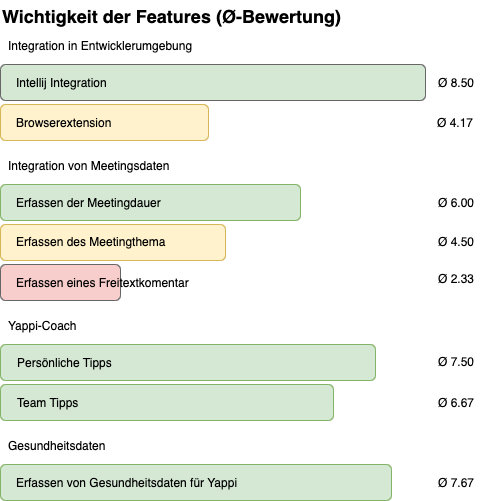
\includegraphics[width=0.85\textwidth]{../figures/konzept-eval-feature-wichtigkeit.drawio.png}
  \caption{Durchschnittsbewertung der Konzeptfunktionen auf einer Likert-Skala von 0 = sehr unwichtig bis 10 = sehr wichtig.}
  \label{fig:konzept-eval-feature-wichtigkeit}
\end{figure}

Die Abbildung~\ref{fig:konzept-eval-feature-wichtigkeit} zeigt die nach Themen gruppierten Durchschnittsbewertungen.
Am höchsten bewertet wurden Funktionen mit direkter Integration in den Arbeitsfluss, wie das IntelliJ-Plugin (8,50)
oder die Erfassung von Gesundheitsdaten (7,67).
Niedrigere Werte erhielten Funktionen, die manuelle Eingaben erfordern, insbesondere Freitextkommentare zu Meetings (2,33).

Die Umfrage diente nicht nur der Bestätigung der Konzeptideen, sondern auch der Priorisierung und Optimierung einzelner Funktionen.
So ergab sich aus den Rückmeldungen, dass die Meetingumfrage als kompakter Frageblock mit Auswahloptionen gestaltet wird,
während Freitextfelder nur ergänzend zum Einsatz kommen.
Damit wird der Aufwand für die Teilnehmenden reduziert und die Wahrscheinlichkeit für regelmässige Rückmeldungen erhöht.

\chapter{Implementierung}
\todo{Einleitung}

\section{Zugriffskontrolle über API-Keys}

    Das API-Key-System dient der sicheren und eindeutigen Authentifizierung externer Dienste gegenüber der \texttt{Yappi-Companion}-API.
    Anstelle von Benutzeranmeldedaten verwenden Clients einen statisch generierten API-Key, der für den jeweiligen Nutzer erstellt und ausschliesslich diesem zugeordnet ist.
    Dies ermöglicht den kontrollierten Zugriff auf geschützte Endpunkte, ohne dass sensible Login-Daten offengelegt oder dauerhaft gespeichert werden müssen.

    Über einen gültigen API-Key können autorisierte Clients Anfragen an Endpunkte mit dem Pfadpräfix \texttt{/companion/} stellen.
    Beispielsweise kann der Fragenblock mit der ID~\texttt{1} wie folgt abgerufen werden:

    \begin{verbatim}
        GET https://yappi.dev/companion/questionblocks/1
        X-API-KEY: <api-key>
    \end{verbatim}


    \subsubsection{Datenbank}
    Die Tabelle \texttt{api\_key} speichert die Metadaten und API-Keys.

    \begin{table}[!htbp]
    \centering
    \begin{tabular}{|l|l|p{9cm}|}
    \hline
    \textbf{Spalte} & \textbf{Datentyp} & \textbf{Beschreibung} \\
    \hline
    \texttt{id} & SERIAL & Primärschlüssel, auto-inkrementierend \\
    \texttt{user\_id} & INTEGER & Fremdschlüssel auf \texttt{users.id} \\
    \texttt{hashed\_key} & TEXT & Gesalteter Hash des API-Keys (z.\,B. BCrypt oder Argon2) \\
    \texttt{created\_at} & TIMESTAMPTZ & Zeitpunkt der Erstellung des Keys \\
    \texttt{expires\_at} & TIMESTAMPTZ & Optionales Ablaufdatum \\
    \texttt{active} & BOOLEAN & Aktivierungs-Flag, um Keys ohne Löschung zu sperren \\
    \hline
    \end{tabular}
    \caption{Schema der Tabelle \texttt{api\_key}}
    \label{tab:api_key_schema}
    \end{table}

    \subsubsection{Backend-Komponenten}
    \begin{itemize}
      \item \textbf{Entität} (\texttt{ApiKey.java}) - Abbildung der Tabelle \texttt{api\_key} als JPA-Entität, ohne Feld für den rohen Key.
      \item \textbf{Repository} (\texttt{ApiKeyRepository.java}) - Zugriff auf API-Key-Datensätze, inkl. Suche nach Key-Präfix.
      \item \textbf{Util-Klasse} (\texttt{ApiKeyUtil.java}) - Generierung zufälliger Keys, Trennung von Präfix und geheimem Teil, Hashing des geheimen Teils mit einem sicheren Algorithmus.
      \item \textbf{Service} (\texttt{ApiKeyService.java}) - Erstellung, Speicherung und Validierung von Keys.
      \item \textbf{Controller} (\texttt{ApiKeyController.java}) - REST-Endpunkte zur Verwaltung von Keys.
    \end{itemize}

    \subsubsection{API-Endpunkte}
    Basispfad: \texttt{/apikey}. Alle Endpunkte setzen einen gültigen JWT im \texttt{Authorization}-Header voraus (\texttt{Bearer <token>}).

    \begin{itemize}
      \item \texttt{GET /apikey} \\
            Liefert den aktiven API-Key des aktuell authentisierten Nutzers als Metadatenobjekt (kein Klartext-Key). \\
            \textbf{Antworten:} \texttt{200 OK}, \texttt{404 Not Found} (kein aktiver Key), \texttt{401 Unauthorized} (fehlender/ungültiger Header).
      \item \texttt{POST /apikey/generate} \\
            Erzeugt einen neuen API-Key für den authentisierten Nutzer und gibt den Klartext-Key einmalig zurück. \\
            \textbf{Antworten:} \texttt{200 OK}, \texttt{401 Unauthorized}.
    \end{itemize}

    \noindent
    \textbf{Nutzung geschützter Ressourcen:} Externe Clients authentisieren sich anschliessend mit \texttt{X-API-KEY: <key>} gegenüber den Companion-/Backend-Endpunkten. Der Klartext-Key wird nicht gespeichert; in der Datenbank liegt nur \texttt{hashed\_key}.

    \noindent
    \textbf{Beispiel (cURL):}
    \begin{verbatim}
    # Key erzeugen
    curl -H "Authorization: Bearer <JWT>" -X POST https://<host>/apikey/generate

    # Aktiven Key (Metadaten) abrufen
    curl -H "Authorization: Bearer <JWT>" https://<host>/apikey
    \end{verbatim}

    \subsubsection{Verarbeitungslogik}//
    \textbf{Erstellung:}
    \begin{enumerate}
      \item Generierung eines neuen Keys (Präfix + geheimer Teil).
      \item Hashing des geheimen Teils.
      \item Speicherung des Hashes und der Metadaten in der Tabelle \texttt{api\_key}.
      \item Rückgabe des vollständigen Keys an den Client (nur einmalig).
    \end{enumerate}
    \textbf{Validierung:}
    \begin{enumerate}
      \item Extraktion des Präfixes und geheimen Teils aus dem API-Key-Header.
      \item Abruf des Datensatzes anhand des Präfixes.
      \item Prüfung auf Existenz, Aktivstatus und Ablaufdatum.
      \item Vergleich des Hashes mit dem übergebenen geheimen Teil.
      \item Bei Erfolg: Authentifizierung des zugehörigen Benutzers.
    \end{enumerate}

    \subsubsection{Sicherheitsintegration}
    \begin{itemize}
      \item \textbf{ApiKeyFilter} - Spring-Security-Filter, der den API-Key aus dem \texttt{X-API-KEY}-Header ausliest und validiert.
      \item \textbf{SecurityConfig} - Bindet den Filter vor dem \texttt{UsernamePasswordAuthenticationFilter} in die Filterkette ein, um API-Key-Anfragen vor anderen Authentifizierungsmethoden zu prüfen.
    \end{itemize}

    \subsubsection{Vorteile}
    \begin{itemize}
      \item Schlüssel werden nie im Klartext gespeichert.
      \item Flexible Verwaltung durch Ablaufdaten und Aktivierungs-Flag.
      \item Sichere Hashing-Verfahren verhindern Missbrauch bei Datenbankkompromittierung.
    \end{itemize}


    \todo{Quelle für spring Securtiy Architektur}
    https://docs.spring.io/spring-security/reference/servlet/architecture.html \\
    \todo{Security "Workarround" erklären}
    \todo{Front End Anpassung}

%--------------------------------------------------------------------------------------------------------------------------------------

\section{IntelliJ IDEA Companion}

\todo{}

\xeno{rework oder}
\gideon{:)}

Yappi wird direkt in die integrierte Entwicklungsumgebung (IDE) eingebunden, um den Arbeitsfluss von Entwicklerinnen
und Entwicklern nicht zu unterbrechen.Als primäre Zielplattform eignet sich ein Plugin für IntelliJ IDEA,
eine der weltweit am häufigsten genutzten Java-Entwicklungsumgebungen von JetBrains.
Die Wahl von IntelliJ IDEA basiert auf drei Hauptfaktoren: hohe Verbreitung im professionellen Java-Umfeld,
umfangreiche Plugin-Schnittstellen zur Integration externer Funktionen und Unterstützung mehrerer Programmiersprachen
und Build-Systeme, was den Einsatz auch in heterogenen Entwicklungsteams ermöglicht.
Die unmittelbare Einbettung in die gewohnte Arbeitsoberfläche erlaubt die Erfassung von Zufriedenheitsdaten ohne Kontextwechsel.

Die Integration trägt dazu bei, den Flow-Zustand zu erhalten.
Flow bezeichnet einen Zustand tiefer Konzentration, der nur entsteht, wenn Anforderungen und Fähigkeiten
im Gleichgewicht stehen und Unterbrechungen vermieden werden.
Kontextwechsel zu externen Tools oder Browsern können diesen Zustand unterbrechen und damit Produktivität sowie Zufriedenheit verringern.
Das IntelliJ-Plugin reduziert solche Unterbrechungen, indem es Feedbackprozesse unmittelbar in den bestehenden Arbeitskontext integriert.

Eine Post-Commit-Aktion ermöglicht es, direkt nach einem abgeschlossenen Commit ein kurzes Feedback abzugeben.
Dadurch entfällt der Umweg über die Webplattform von Yappi, was die Bedienung beschleunigt und die Gefahr von Befragungsmüdigkeit verringert.
Kurze, kontextbezogene Abfragen im richtigen Moment erhöhen die Teilnahmebereitschaft und verbessern die Datenqualität.

Ziel ist ein Erfassungsprozess, der unauffällig, effizient und vollständig in den Entwicklungsprozess integriert ist


%--------------------------------------------------------------------------------------------------------------------------------------


\section{Calendar Companion}

        Der \textit{Calendar Companion} erweitert die Yappi-Plattform um eine Kalenderintegration mit Echtzeitbenachrichtigung
        und integriertem Feedbackprozess. Er kombiniert Backend-Services, eine Browsererweiterung sowie einen Kommunikationsbroker,
        um Kalendereinträge zu synchronisieren und direktes Feedback zu ermöglichen.

        Zur automatischen Erkennung relevanter Meetings wird eine Anbindung an das Kalendersysteme des Entwickler vorgesehen.
        Wichtig dabei ist es einen Offenen Standard zu verwenden um eine möglichst hohe Kompatibilität mit Kalendersystemen zu schaffen.
        Grundlage dazu bildet das weit verbreitete iCalendar-Format (ICS), das von nahezu allen gängigen Plattformen unterstützt wird.
        Das Konzept sieht vor, dass der Nutzer in Yappi auf seinem Profil den zugriff auf den Kalender hinterlegen kann.
        Regelmässig werden die auf einen vom Nutzer im Kalender erstellten Kalendereinträge in die Datenbank synchronisiert.
        Auf dieser Basis kann die Anwendung automatisch identifizieren, wann ein Meeting stattfindet.
        Dadurch lassen sich Feedback-Anfragen unmittelbar nach dem Ende einer Besprechung auslösen, ohne dass der Nutzer manuell eingreifen muss.

        Die Synchronisation des Kalender erfolgt ausschliesslich lesend, um Eingriffe in persönliche Kalender zu vermeiden.
        Alle übermittelten Kalenderinformationen werden vertraulich behandelt und ausschliesslich für den definierten Zweck genutzt.
        Informationen zu Kalendereinträge sind nur für den Nutzer persönlich einsehbar.

        Durch diese Anbindung entfällt das manuelle Erfassung von Kalendereinträgen. Meetings werden automatisch erkannt,
        Änderungen übernommen und die Nutzer benachrichtigt. So entsteht ein nahtloser integrierter feedback flow um die
        Zufriedenheitsdaten von Meetings für die Entwickler zu erheben.

        Dieses Kapitel beschreibt die technische Implementierung der einzelnen Komponenten, deren Zusammenspiel
        sowie die zugrunde liegenden Datenstrukturen.


        \begin{figure}[!htbp]
          \centering
          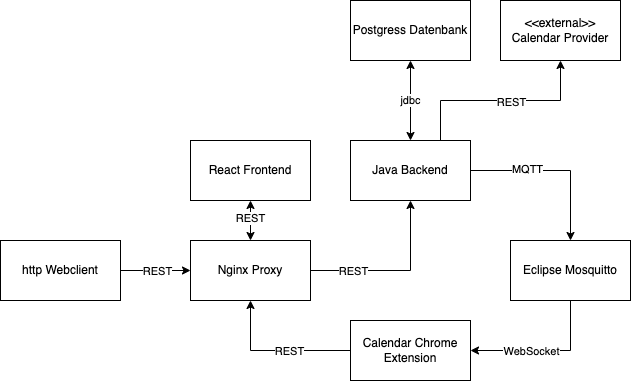
\includegraphics[width=0.85\textwidth]{../figures/implementation-claendar-companion-system.drawio.png}
          \caption{Systemübersicht zur Kalenderintegration in Yappi}
          \label{fig:implementation-calendar-companion-system}
        \end{figure}

        Die Abbildung~\ref{fig:implementation-calendar-companion-system} zeigt eine Systemübersicht der Kalenderintegration.

  \subsection{Yappi Chrome Extension}
      Die Companion-App wird als Browsererweiterung umgesetzt, um eine direkte Interaktion mit den Entwicklern zum richtigen
      Zeitpunkt zu ermöglichen. Nach dem Ende eines im Kalender erfassten Meetings erhält der Nutzer eine Benachrichtigung,
      die zur Abgabe einer kurzen Bewertung auffordert. Diese zeitnahe Erhebung stellt sicher, dass Eindrücke und Wahrnehmungen
      noch frisch sind und die Datenqualität hoch bleibt. Die Interaktion erfolgt freiwillig, um Befragungsmüdigkeit zu vermeiden,
      und ist so gestaltet, dass die Beantwortung wenige Sekunden benötigt. Durch die Integration in den Browser wird kein
      zusätzlicher Systemwechsel nötig, wodurch die Hemmschwelle zur Teilnahme sinkt.

    \subsubsection{Architektur}
        Die Anwendung besteht aus zwei Hauptkomponenten:
        \begin{enumerate}
          \item \textbf{Persistenter Background-Prozess}
                Läuft dauerhaft im Hintergrund und ist für die Kommunikation mit dem Eclipse Mosquitto Nachrichtenbroker, die Verwaltung des Zustands
                und das proaktive Benachrichtigen des Nutzers zuständig.
          \item \textbf{Temporäre Popup-Benutzeroberfläche (UI)}
                Wird nur bei aktiver Benutzerinteraktion geladen und dient der Darstellung der Benutzeroberfläche sowie dem Erfassen von Feedback.
        \end{enumerate}

    \subsubsection{Komponenten im Detail}
        \textbf{Background-Prozess (\texttt{background/background.js})} \\
            \begin{itemize}
              \item Aufbau und Aufrechterhaltung einer Websockets-Verbindung (über \texttt{lib/mqtt.js}) zum Yappi Kommunikationsbroker.
              \item Abonnieren der benutzerspezifischen Topics zur Echtzeitbenachrichtigung (\texttt{companion/event/calendar/*user-token*}).
              \item Verarbeitung eingehender Nachrichten und Erzeugung nativer Desktop-Benachrichtigungen (\texttt{chrome.notifications}).
              \item Persistente Speicherung der letzten zehn Ereignisse in \texttt{chrome.storage.local} nach FIFO-Prinzip.
            \end{itemize}


        \textbf{Popup-Benutzeroberfläche (\texttt{popup/home.html})} \\
            \begin{itemize}
              \item Dynamischer Umfrage-Builder (\texttt{popup/survey/builder.js}):
                    Ruft aktuelle Umfragen über die REST-API ab, generiert DOM-Elemente aus JSON Vorlagen (\texttt{popup/questionblock.html},
                    \texttt{popup/questionblock.js}) und integriert diese in die Ansicht.
                    Mehr Details dazu in Abschnitt \ref{section:Dynamische Umfragen}.
                    \todo{check link}
              \item Feedback-Übermittlung (\texttt{popup/popup.js}):
                    Sammelt Antworten, strukturiert sie als JSON und sendet sie per POST-Request an das Yappi-Backend.
            \end{itemize}


    \subsubsection{Benutzeroberfläche (UI)}
        Die Benutzeroberfläche der Yappi Chrome Extension besteht aus zwei zentralen Interaktionselementen: Systembenachrichtigungen und der Popup-Ansicht im Browser.

        \textbf{Systembenachrichtigungen} \\
            Beim Ende eines Events im Kalender des Benutzer, erzeugt die Extension eine native Systembenachrichtigung siehe Abbildung \ref{fig:yappi-extension-notification}.
            Diese Benachrichtigungen enthalten:
            \begin{itemize}
                \item Titel und Beschreibung des Meetings (z.\,B. \glqq Meeting IP5 - Standup\grqq),
                \item Uhrzeit des Termins,
                \item das Yappi-Logo als Icon,
                \item interaktive Schaltflächen wie \texttt{Review Event} zur direkten Abgabe von Feedback.
            \end{itemize}
            Durch diese direkte Interaktionsmöglichkeit kann Feedback ohne Umweg über die Hauptanwendung erfasst werden.

            \begin{figure}[htbp]
              \centering
              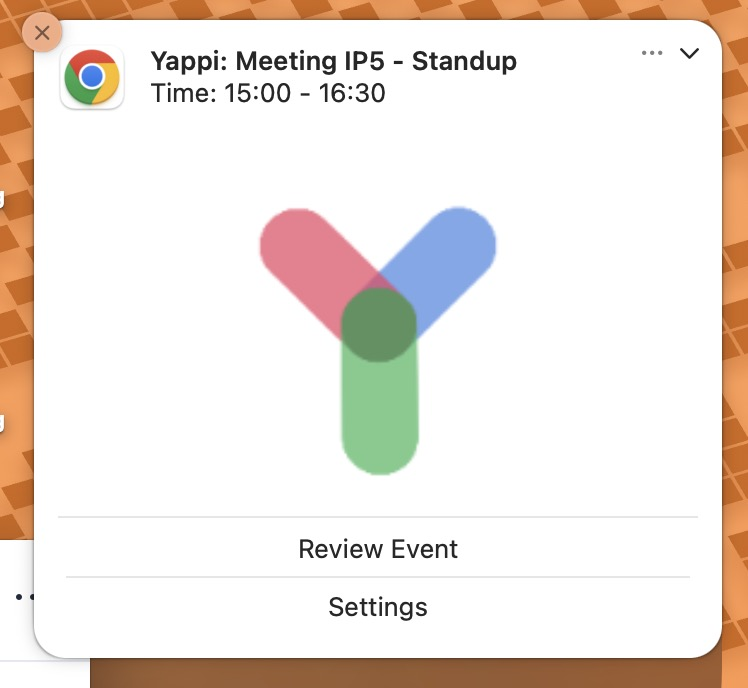
\includegraphics[width=0.60\textwidth]{../figures/yappi-chrome-extension/yappi-extension-notification.jpg}
              \caption{Systembenachrichtigung der Chrome Erweiterung in macOS}
              \label{fig:yappi-extension-notification}
            \end{figure}


        \textbf{Popup-Ansicht} \\
            Das Browser-Popup siehe Abbildung \ref{fig:yappi-extension-popup} dient als Haupt-UI der Extension und wird durch einen
            Klick auf das Yappi-Icon in der Browser-Toolbar geöffnet.
            Die Ansicht enthält:
            \begin{itemize}
                \item Verbindungsstatus zum Nachrichtenbroker,
                \item Benutzerhinweis zum erfolgreichen Setup,
                \item eine Liste kürzlich abgeschlossener Meetings zu welchen noch kein Feedback gegeben wurde,
                \item Aktionsbuttons für jedes Meeting:
                    \begin{itemize}
                        \item \texttt{Review} Öffnet die zugehörige Feedback-Umfrage.
                        \item \texttt{Delete} Entfernt den Eintrag aus der Liste der letzten Meetings.
                    \end{itemize}
            \end{itemize}
            Das Design stellt sicher, dass Benutzer sowohl über Echtzeitbenachrichtigungen als auch über die Popup-Ansicht
            jederzeit auf anstehende Feedback-Aufgaben zugreifen können.

            \begin{figure}[!htbp]
              \centering
              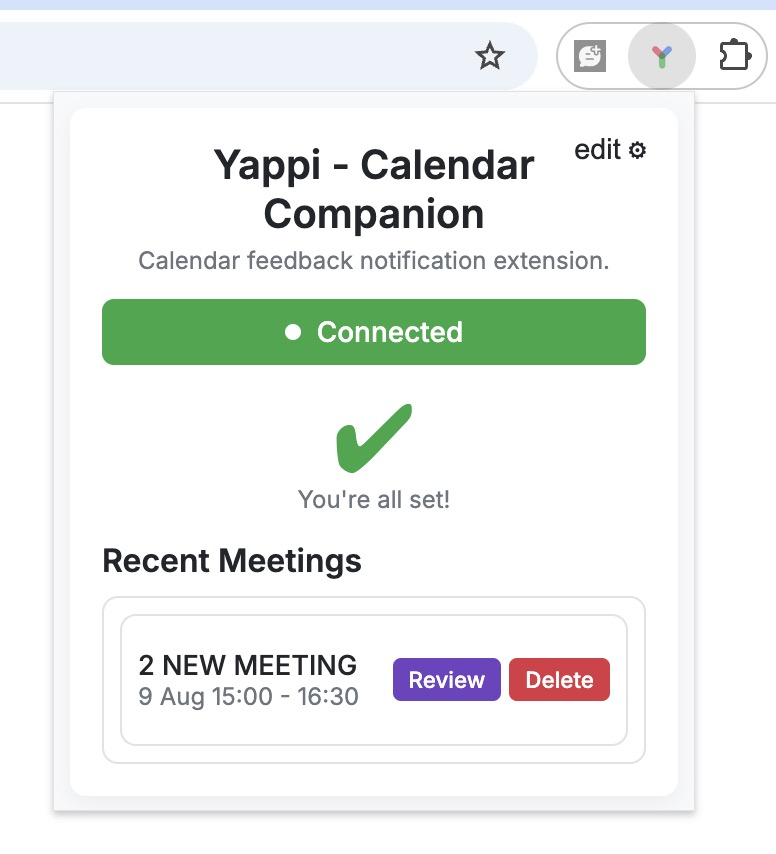
\includegraphics[width=0.60\textwidth]{../figures/yappi-chrome-extension/yappi-extension-popup.jpg}
              \caption{Benutzeroberfläche der Chrome Erweiterung}
              \label{fig:yappi-extension-popup}
            \end{figure}


    \subsubsection{Kommunikationskanäle}
      \todo{grafik zu kommunikation}
        Die Verbindung zum Yappi-Backend erfolgt über zwei Kommunikationskanäle:
        \begin{itemize}
          \item \textbf{REST-API} Für synchronen Abruf von Daten und Übermittlung von Antworten.
          \item \textbf{MQTT-Broker} Für asynchrone Benachrichtigungen in Echtzeit.
        \end{itemize}

        Die interne Kommunikation zwischen Background-Prozess und Popup-UI nutzt die Browser-API \texttt{chrome.storage}.
        Dort werden alle Informationen, wie Clientdaten oder die letze Kalenderevents gespeichert und ausgetauscht.



    \subsubsection{Externe Abhängigkeiten}
        \begin{itemize}
          \item \textbf{Yappi-Backend} Bereitstellung der REST-API und MQTT-Broker.
          \item \textbf{MQTT.js} (\texttt{lib/mqtt.js}) JavaScript-Clientbibliothek für MQTT-Kommunikation.
        \end{itemize}

\subsection{Backend-Integration}

        Das Yappi-Backend fungiert als Zentraler Controller der gesamten Kalenderintegration von Yappi.
        Es ist zuständig für jeglichen Datenaustausch, Datenspeicherung sowie Datenverarbeitung und besteht
        aus verschiedenen modulen welche alle ihre verantwortlichkeiten haben.

        Für den Calendar Companion wurde ein eigenes Modul erstellt.

        Das Kalendermodul im Yappi-Backend ist für die Verwaltung und Bereitstellung von Kalendereinträgen verantwortlich.
        Es unterstützt sowohl den Abruf von Einträgen über eine REST-API als auch eine proaktive Benachrichtigung der Chrome-Extension in Echtzeit.
        Letzteres erfolgt über das Publish-Subscribe-Protokoll \textit{MQTT} (Message Queuing Telemetry Transport).
        Zudem ist es Zuständig für das Laden und synchronisieren der externen iCalendar-Daten (ICS) welche von den Nutzer hinterlegt werden.


    \subsubsection{Model-Klasse}
        Die zentrale Datenstruktur bildet die JPA-Entität \texttt{CalendarEvent.java} (\texttt{entities/}).
        Sie repräsentiert einen einzelnen Kalendereintrag mit Attributen wie \texttt{title}, \texttt{startDate}, \texttt{endDate}, \texttt{allDay} sowie der Zuordnung zu einem Nutzer (\texttt{userId}).
        Diese Klasse wird innerhalb des Backends zwischen Services und Controllern verwendet.

    \subsubsection{API-Endpunkte (\texttt{CalendarController})}
        Die Interaktion externer Clients mit dem Kalendermodul erfolgt über folgende REST-Endpunkte:
        \begin{itemize}
            \item \texttt{GET /api/calendar/\{userId\}}
                Ruft alle Kalendereinträge einer bestimmten Nutzer-ID ab.
                Der Controller delegiert die Anfrage an den \texttt{CalendarService}, der die Daten lädt und als JSON zurückgibt.
            \item \texttt{POST /api/calendar/sync}
                Stösst die Synchronisation manuell an, z.\,B. für sofortige Aktualisierungen oder Debugging.
                Nutzt dieselbe Logik wie die automatische Synchronisation durch den \texttt{CalendarEventScheduler}.
        \end{itemize}

    \subsubsection{Service-Schicht (\texttt{CalendarService})}
        Der \texttt{CalendarService} enthält die Geschäftslogik und entkoppelt Controller und geplante Aufgaben von der Datenverarbeitung.
        Er übernimmt:
        \begin{itemize}
            \item Abruf von Kalendereinträgen,
            \item Erstellung und Aktualisierung von Einträgen durch Abgleich mit externen Daten,
            \item Benachrichtigung über \texttt{MQTT} nach dem Ende von Terminen.
        \end{itemize}

    \subsubsection{Geplante Aufgaben (\texttt{CalendarEventScheduler})}
        Zwei periodische Jobs sorgen für Aktualität und Benachrichtigungen:
        \begin{enumerate}
            \item \textbf{Prüfung beendeter Events} (alle 60 Sekunden):
                Erkennt neu abgeschlossene Kalendereinträge und benachrichtigt betroffene Clients über \texttt{MQTT}.
            \item \textbf{Kalendersynchronisation} (alle 5 Minuten):
                Aktualisiert Kalendereinträge auf Basis externer ICS-Daten.
                Dabei werden neue Events erstellt, geänderte aktualisiert und nicht mehr vorhandene gelöscht.
                Änderungen lösen eine Update-Benachrichtigung an die Clients aus.
        \end{enumerate}

    \subsubsection{Echtzeit-Benachrichtigungen (\texttt{MqttService})}
        Nach Änderungen publiziert der \texttt{MqttService} Nachrichten auf themenspezifischen Topics (z.\,B. \texttt{deardev/teams/\{teamId\}/calendar}).
        Clients abonnieren diese Topics und können ihre UI unmittelbar aktualisieren, ohne Polling durchführen zu müssen.


\subsection{Datenbankerweiterung}

        Zur Speicherung der Kalendereinträge wurde die neue Tabelle \texttt{calendar\_events} eingeführt.
        Die Struktur wird durch die JPA-Entität \texttt{CalendarEvent.java} definiert.

    \begin{table}[!htbp]
        \centering
        \begin{tabular}{|l|l|p{9cm}|}
            \hline
                \textbf{Spalte} & \textbf{Datentyp} & \textbf{Beschreibung} \\
            \hline
                \texttt{id} & INTEGER & Primärschlüssel des Eintrags \\
                \texttt{title} & VARCHAR & Titel des Kalenderevents (z.\,B. \glqq Sprint~1\grqq) \\
                \texttt{start\_date} & TIMESTAMP & Startdatum und -zeit \\
                \texttt{end\_date} & TIMESTAMP & Enddatum und -zeit \\
                \texttt{all\_day} & BOOLEAN & Kennzeichen für ganztägige Events \\
                \texttt{user\_id} & INTEGER & Fremdschlüssel zur Tabelle \texttt{users} \\
                \texttt{team\_id} & INTEGER & Fremdschlüssel zur Tabelle \texttt{teams} \\
            \hline
        \end{tabular}
        \caption{Schema der Tabelle \texttt{calendar\_events}}
        \label{tab:calendar_events_schema}
    \end{table}

    \subsubsection{Backend-Komponenten}
        \begin{itemize}
            \item \textbf{Entität} (\texttt{CalendarEvent.java}): Datenmodell und Tabellenstruktur.
            \item \textbf{Repository} (\texttt{CalendarEventRepository.java}): CRUD-Operationen auf \texttt{calendar\_events}.
            \item \textbf{Service} (\texttt{CalendarService.java}): Geschäftslogik zum Erstellen, Abrufen und Löschen von Events.
            \item \textbf{Controller} (\texttt{CalendarController.java}): REST-Endpunkte zum Abrufen von Events pro Nutzer.
            \item \textbf{Scheduler} (\texttt{CalendarEventScheduler.java}): Zeitgesteuerte Erstellung und Aktualisierung der Events.
            \item \textbf{Factory} (\texttt{CalendarEventFactory.java}): Hilfsklasse zur einfachen Erstellung neuer Eventobjekte.
        \end{itemize}

    \subsubsection{Automatisierte Erstellung}
        Der \texttt{CalendarEventScheduler} generiert automatisch Einträge auf Basis aktiver Sprints:
        \begin{enumerate}
            \item Abruf aller aktiven Sprints für jedes Team,
            \item Prüfung, ob für jedes Teammitglied bereits ein Event existiert,
            \item Erstellung neuer Events mittels \texttt{CalendarEventFactory}, falls erforderlich,
            \item Speicherung der Events über das \texttt{CalendarEventRepository}.
        \end{enumerate}

\subsection{Kommunikationsbroker}
        Für die Echtzeitübertragung von Benachrichtigungen an Clients wird der Open-Source-MQTT-Broker \textbf{Eclipse Mosquitto} eingesetzt.
        \textit{MQTT} (Message Queuing Telemetry Transport) ist ein leichtgewichtiges Publish-Subscribe-Protokoll, das sich besonders für Anwendungen mit geringer Latenz und hohem Aktualisierungsbedarf eignet.

    \subsubsection{Zweck}
        Der Kommunikationsbroker ermöglicht die sofortige Benachrichtigung von Companion-Anwendungen, insbesondere der Google-Chrome-Erweiterung des Calendar Companions.
        Damit entfällt die Notwendigkeit von Polling-Anfragen an das Backend, was die Netzwerklast reduziert und eine reaktive Benutzeroberfläche ermöglicht.

    \subsubsection{Kommunikationsfluss}
        \begin{enumerate}
            \item Das Backend erkennt eine relevante Änderung, z.\,B. das Ende eines Meetings oder die Erstellung eines neuen Kalendereintrags.
            \item Der \texttt{MqttService} des Backends verbindet sich mit dem Mosquitto-Broker und publiziert die Nachricht auf einem benutzerspezifischen Topic:
                \texttt{calendar/event/\{user-api-key\}}.
            \item Die Chrome-Erweiterung des Calendar Companions ist als MQTT-Client auf diesem Topic angemeldet (\textit{subscribed}).
            \item Beim Empfang einer Nachricht aktualisiert der Client die lokale Ansicht und kann bei Bedarf Folgeaktionen anstossen (z.\,B. Anzeige eines Feedback-Dialogs).
        \end{enumerate}

    \subsubsection{Nachrichtenformat}
        Die vom Backend publizierten Benachrichtigungen werden als JSON-Objekte gesendet.
        Eine typische Nachricht enthält die folgenden Felder:

        \begin{verbatim}
            {
                "eventId": 3002,
                "userId": 1,
                "title": "Meeting IP5 - Standup",
                "startDate": "2025-08-09T15:00",
                "endDate": "2025-08-09T15:15",
                "location": "",
                "questionBlockId": 1,
                "teams": [
                    {
                        "id": 1,
                        "name": "Test Team 1"
                    },
                    {
                        "id": 3,
                        "name": "Test Team 2"
                    }
                ]
            }
        \end{verbatim}

    \subsubsection{Vorteile}
        \begin{itemize}
            \item Sofortige Zustellung ohne Polling.
            \item Geringe Netzwerklast durch Publish-Subscribe-Architektur.
            \item Einfaches Routing über benutzerspezifische Topics.
            \item Erweiterbar für weitere Eventtypen oder Companion-Anwendungen.
        \end{itemize}



\subsection{Dynamische Umfragen}
    Die dynamischen Umfragen in Yappi basieren auf flexibel konfigurierbaren Fragenblöcken, die als JSON-Objekte in der Datenbank gespeichert werden.
    Diese Struktur ermöglicht es, Umfragen anzupassen oder zu erweitern, ohne Änderungen am Anwendungscode vorzunehmen.

    \subsubsection{Datenbank}
        Die Tabelle \texttt{questionblocks} speichert die Konfiguration einzelner Fragenblöcke.

        \begin{table}[!htbp]
            \centering
            \begin{tabular}{|l|l|p{9cm}|}
                \hline
                    \textbf{Spalte} & \textbf{Datentyp} & \textbf{Beschreibung} \\
                \hline
                    \texttt{id} & SERIAL & Eindeutiger, automatisch inkrementierender Primärschlüssel \\
                    \texttt{configuration} & JSONB & Vollständige Konfiguration des Fragenblocks als JSON-Objekt.
                    Ermöglicht flexible Strukturierung und effiziente Abfragen \\
                \hline
            \end{tabular}
            \caption{Schema der Tabelle \texttt{questionblocks}}
            \label{tab:questionblocks_schema}
        \end{table}

        \noindent
        \textbf{Anmerkung:} Der Datentyp \texttt{JSONB} (Binary JSON) erlaubt eine performante Speicherung und gezielte Abfragen innerhalb der JSON-Daten.

    \subsubsection{Backend-Komponenten}
        \begin{itemize}
            \item \textbf{Entität} (\texttt{QuestionBlock.java}) - Abbildung der Tabelle \texttt{questionblocks} als JPA-Entität.
                Attribute: \texttt{id} (INTEGER) und \texttt{configuration} (\texttt{JsonNode}).
            \item \textbf{Repository} (\texttt{QuestionBlockRepository.java}) - CRUD-Operationen auf der Tabelle.
            \item \textbf{Service} (\texttt{QuestionBlockService.java}) - Geschäftslogik für den Zugriff und die Validierung von Fragenblöcken.
            \item \textbf{Controller} (\texttt{QuestionBlockController.java}) - Bereitstellung der API-Endpunkte.
        \end{itemize}

    \subsubsection{API-Endpunkte}
        \begin{itemize}
            \item \texttt{GET /companion/questionblocks/\{id\}}
                Ruft den Fragenblock mit der angegebenen ID ab.
                \textbf{Antworten:} \texttt{200 OK} mit JSON-Objekt oder \texttt{404 Not Found}, falls nicht vorhanden.
        \end{itemize}

    \subsubsection{Darstellung in der Companion-App}
        Die Chrome Extension ruft den entsprechenden Fragenblock per REST-API ab.
        Das Skript \texttt{popup/survey/builder.js} parst die JSON-Daten und erstellt für jede Frage die passenden HTML-Elemente
        basierend auf den Templates (\texttt{popup/questionblock.html}) und der Logik in \texttt{popup/questionblock.js}.
        Unterstützt werden Fragetypen wie:
        \begin{itemize}
            \item Likert-Skalen
            \item Single-Choice
            \item Multiple-Choice
            \item Freitext
        \end{itemize}

    \subsubsection{Beispiel Fragebogen}
        Das UI des Fragebogen ist sehr einfach gehalten. In der Abbildung \ref{fig:yappi-extension-feedback} ist eine Grafische-Darstellung
        einer Beispielumfrage zu sehen.

        \begin{figure}[!htbp]
          \centering
          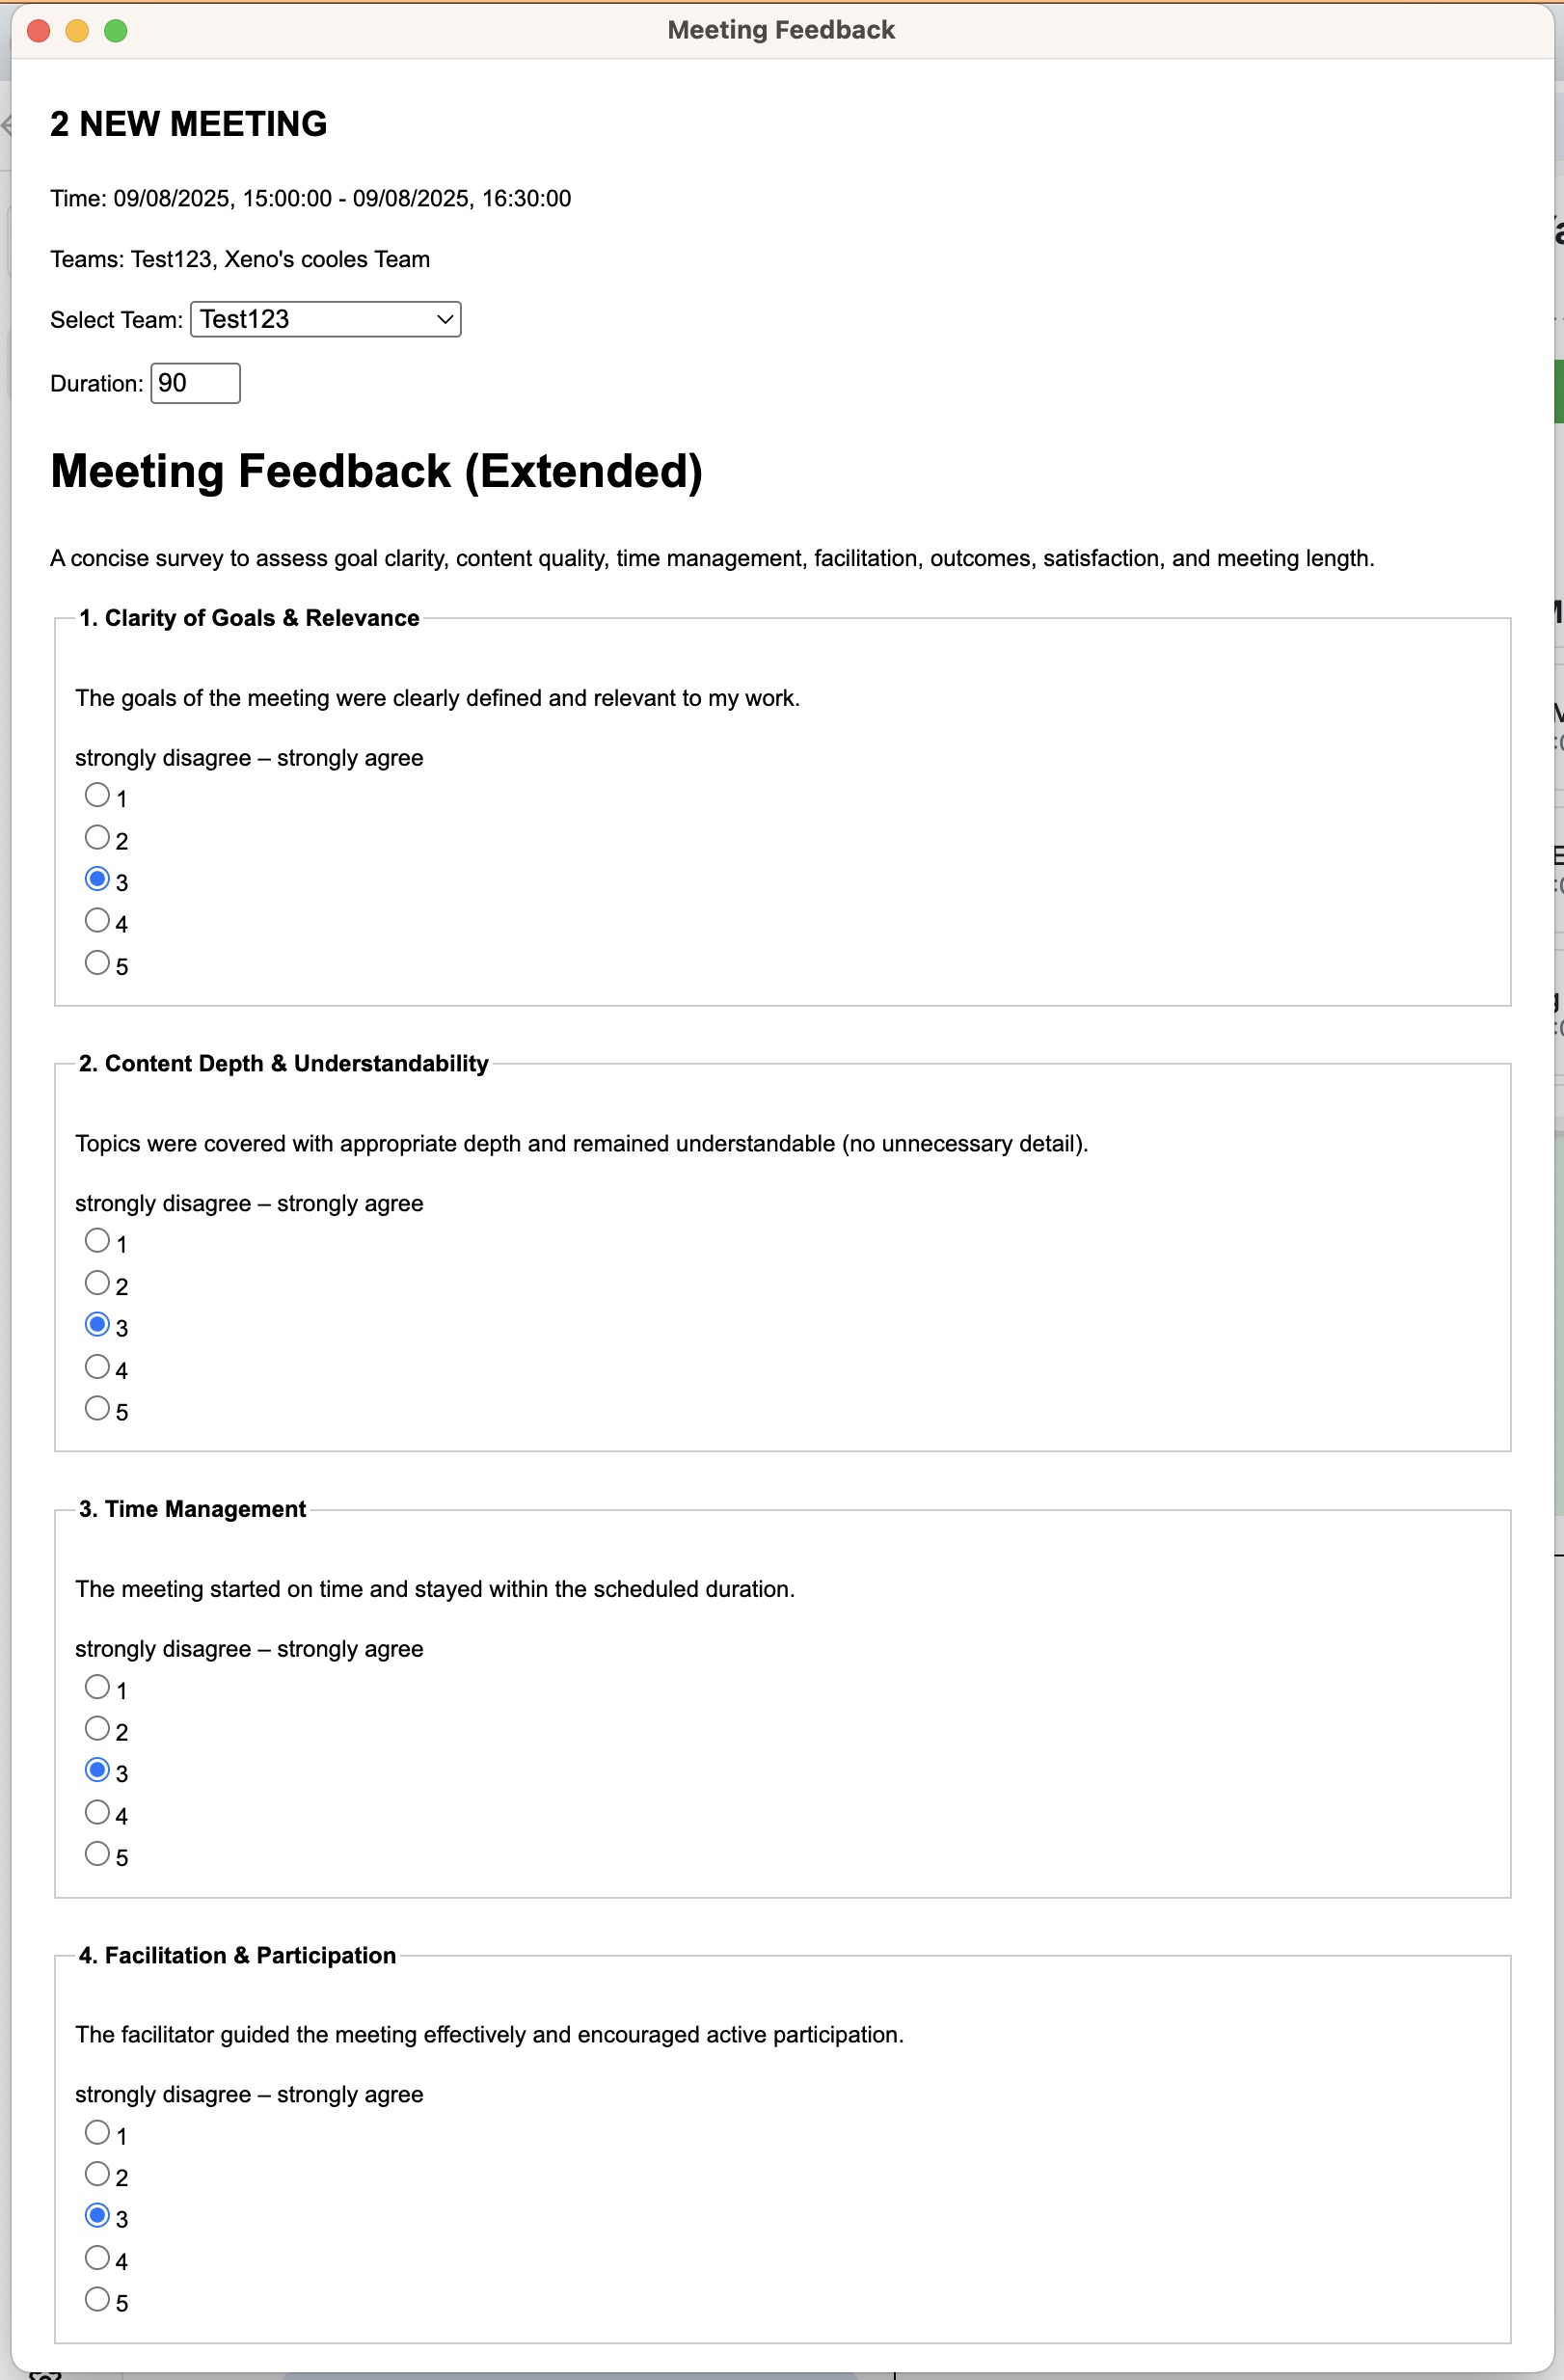
\includegraphics[width=0.90\textwidth]{../figures/yappi-chrome-extension/yappi-extension-feedback.jpg}
          \caption{Feedbackformular zu Kalenderevent}
          \label{fig:yappi-extension-feedback}
        \end{figure}

        Die Konfiguration des Fragebogen kann aus folgender JSON Struktur abgeleitet werden.

        \begin{verbatim}
            {
            "id": "1000",
            "title": "Basic Meeting Feedback",
            "description": "This is am Meeting feedback survey.",
            "sections": [
            {
                "id": "q1",
                "type": "likert",
                "title": "1. Clarity of Goals & Relevance",
                "prompt": "The goals of the meeting were clearly defined.",
                "required": true,
                "min": 1,
                "label_min": "strongly disagree",
                "max": 5,
                "label_max": "strongly agree",
                "step": 1,
                "default": 3
            },
            {
                "id": "q2",
                "type": "single-choice",
                "title": "2. Meeting Length",
                "prompt": "How would you rate the length of the meeting?",
                "required": true,
                "options": [
                    { "value": "too-short", "label": "Too short" },
                    { "value": "just-right", "label": "Just right" },
                    { "value": "too-long", "label": "Too long" }
                ],
                "default": "just-right"
            },
            {
            "id": "q3",
            "type": "multiple-choice",
            "title": "3. Meeting Highlights",
            "prompt": "Which aspects of the meeting did you find valuable? (Select all that apply)",
            "required": false,
            "options": [
                { "value": "clear-agenda", "label": "Clear agenda" },
                { "value": "useful-content", "label": "Useful content" },
                { "value": "good-discussion", "label": "Good discussion" },
                { "value": "action-items", "label": "Clear action items" }
            ],
            "default": ["clear-agenda", "good-discussion"]
            },
            {
                "id": "q5",
                "type": "free-text",
                "title": "4. Additional Comments",
                "prompt": "Please share any additional feedback or suggestions.",
                "required": false,
                "placeholder": "Type your feedback here...",
                "maxLength": 500
            }
            ]
            }
        \end{verbatim}

    \subsubsection{Vorteile}
        \begin{itemize}
            \item Anpassung und Erweiterung von Umfragen ohne Codeänderungen.
            \item Unterstützung verschiedener Fragetypen und Layouts.
            \item Zentrale Verwaltung und Wiederverwendung von Fragenblöcken.
        \end{itemize}


\todo{Sequenzdiagramm}
\todo{Front End Anpassung}
% Die bestehenden Funktionen von Yappi werden um einen Bereich zur Meetinganalyse ergänzt.
% Entwickler sehen hier ihre eigenen Feedbackabgaben und offene Anfragen.
% Auf der Teamebene kann auf aggregierte, anonymisierte Auswertungen zu den Meetings ihres Teams zugegriffen werden.
% Die Konfiguration der Kalenderintegration und der Verbindung zur Companion-App wird im Nutzerprofil zentral verwaltet.
% Dadurch bleibt die Erweiterung vollständig in die bestehende Systemarchitektur eingebettet und benötigt keine separaten Plattformen.

% \subsubsection{Datenverarbeitung und Auswertung}
%
% Die erhobenen Feedbackdaten werden ausschliesslich auf dem Yappi-Server verarbeitet.
% Vor der Auswertung erfolgt eine Anonymisierung, um Rückschlüsse auf einzelne Personen zu verhindern.
% Für jedes Meeting werden aggregierte Kennzahlen, wie Durchschnittswerte der sieben Kriterien oder Verteilungen der Bewertungen, berechnet.
% Diese werden nur dann angezeigt, wenn eine vordefinierte Mindestanzahl an Rückmeldungen vorliegt.
% Neben der Auswertung einzelner Meetings können über längere Zeiträume Trends analysiert und Optimierungsmassnahmen evaluiert werden.

%--------------------------------------------------------------------------------------------------------------------------------------

\section{Health Companion}

Gesundheitsdaten können wertvolle Zusatzinformationen zur Entwicklerzufriedenheit liefern. Sie ergänzen subjektive Stimmungsangaben
um objektive Messwerte, die Rückschlüsse auf Belastung und Erholung ermöglichen. Durch die Anbindung an etablierte Schnittstellen
wie Apple Health Kit oder Garmin Health API lassen sich Metriken wie Schlafqualität, Herzfrequenz oder Stressindikatoren
automatisiert erfassen. Diese Daten bilden zusammen mit den Prozess- und Zufriedenheitsmetriken eine erweiterte Grundlage, um
Korrelationen zwischen physischem Wohlbefinden und Arbeitszufriedenheit zu erkennen und gezielte Massnahmen abzuleiten.

\subsection{Quellen und Schnittstellen für Gesundheitsdaten}

Für die Integration von Gesundheitsdaten wurden mehrere Optionen geprüft. Im Mittelpunkt standen die Garmin Health API sowie Apple
Health Kit. Beide Quellen decken relevante Metriken wie Schritte, Herzfrequenz, Schlaf und Stress/HRV ab, unterscheiden sich jedoch
deutlich hinsichtlich Zugangsmodell, Datenschutzmechanismen, Integrationsaufwand und Eignung für nicht-kommerzielle
Forschungsprojekte.

\begin{description}
  \item[Garmin Health API] Die Garmin Health API stellt über eine REST-Schnittstelle umfangreiche Tages- und Aktivitätsmetriken
    bereit. Die Daten werden in der Regel nach dem Gerätesync via über die Mobile Applikation von Garmin bereitgestellt und in
    JSON ausgeliefert. die Plattform unterstützt Pull- und Push-Modelle, sodass auch eine ereignisgetriebene Integration möglich
    ist. Der Zugang ist für genehmigte Business-Developer vorgesehen. Für die kommerzielle Nutzung fallen in der Regel
    Lizenzgebühren an. Diese geschäftliche Ausrichtung sowie die erforderliche formale Zulassung machen die direkte Nutzung für
    ein kleines, nicht-kommerzielles Forschungsprojekt unpassend. Zwar existieren Forschungsprogramme und Partnerlösungen rund um
    Garmin, diese sind jedoch üblicherweise an formelle Kooperationen, Vertragsaufwände und teils Kosten gebunden, was die
    Umsetzungshürde erhöht \cite{garmin_healthapi_2025}.
  \item[Apple Health Kit] Health Kit dient auf iOS als zentrales, lokales Datenrepository für Gesundheits- und Fitnessdaten von
    iPhone, Apple Watch und angebundenen Geräten/Apps. Der Zugriff erfolgt feingranular pro Datentyp und erfordert stets explizite
    Nutzerzustimmung (Lesen/Schreiben getrennt). Daten liegen verschlüsselt auf dem Gerät. Apps erhalten nur Zugriff auf die
    explizit freigegebenen Kategorien. Für die Integration stehen dokumentierte APIs und Query-Muster zur Verfügung. Eine
    serverseitige Drittplattform ist nicht erforderlich, wodurch Architektur, Betrieb und Datenschutzfolgenabschätzung vereinfacht
    werden \cite{apple_healthkit_2025}.
\end{description}

Da die Garmin Health API primär für kommerzielle Anwendungen vorgesehen ist und der beantragte Zugang für dieses Projekt nicht
gewährt wurde, wurde Apple Health Kit als geeignetere Datenquelle ausgewählt. Für die Umsetzung bedeutet dies, dass eine
iOS-Anwendung entwickelt wird, die die relevanten Daten aus Apple HealthKit ausliest und an Yappi überträgt.

\subsection{Daten aus HealthKit auslesen}
\todo{}

\subsection{Daten an Yappi übertragen}
\todo{}
\subsubsection{Backend}
\todo{}
\subsubsection{Datenbankerweiterung}
\todo{}

\subsection{Benutzeroberfläche der iOS App}
\todo{mit screenshot}

%--------------------------------------------------------------------------------------------------------------------------------------

\section{Deployment und CI/CD}
\todo{ein wieso}

    Das Deployment der Yappi-Plattform erfolgt automatisiert mittels \textit{Continuous Integration/Continuous Deployment}
    (CI/CD) über GitHub Actions. Die Ausführung erfolgt auf einem SwitchEngines-Cloud-Server mit Debian Linux.
    Das System ist vollständig Dockerisiert. Der externe Zugriff wird durch einen NGINX-Reverse-Proxy ermöglicht.

    Ziel ist ein einfaches, schnelles und reproduzierbares Deployment direkt nach der Continuous-Integration-Phase.
    Der Build erzeugt versionierte, unveränderliche Docker-Images, die in ein Repository publiziert und auf
    Zielumgebungen mit Docker Compose oder Kubernetes ausgerollt werden kann. Die Konfiguration erfolgt über
    Umgebungsvariablen, Secrets werden zentral verwaltet. Durch die vollständige Containerisierung bleibt die Lösung
    host-agnostisch und kann mittels Infrastructure as Code (z. B. Terraform) und standardisierten Manifesten
    ohne Codeanpassungen auf neue Hosting-Systeme migriert werden.

    \subsection{Build- und Deployment-Pipeline}

        Für Backend und Frontend bestehen separate GitHub-Actions-Workflows.
        Beide nutzen einen self-hosted GitHub Runner, der direkt auf dem Zielserver installiert ist.
        Die Ausführung der Workflows erfolgt automatisch bei Pushes auf die Branches \texttt{develop}.
        Zusätzlich kann der Prozess manuell über \texttt{workflow\_dispatch} gestartet werden.

        Die Abbildung~\ref{fig:backend-flow} zeigt die einzelnen Schritte des automatisierten Build- und Deployment-Prozesses für das Backend
        (vom Quellcode-Checkout bis zum Neustart der Container).

        \begin{figure}[H]
          \centering
          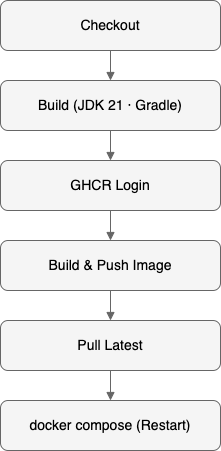
\includegraphics[width=0.3\textwidth]{../figures/backend-flow.drawio.png}
          \caption{Deployment flow vom Backend}
          \label{fig:backend-flow}
        \end{figure}


        Analog dazu veranschaulicht Abbildung~\ref{fig:frontend-flow} den entsprechenden Ablauf für das Frontend,
        inklusive Linting, Next.js-Build und Bereitstellung des Docker-Images.

        \begin{figure}[H]
          \centering
          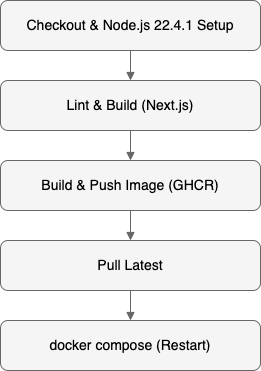
\includegraphics[width=0.3\textwidth]{../figures/frontend-flow.drawio.png}
          \caption{Deployment flow vom Frontend}
          \label{fig:frontend-flow}
        \end{figure}

    \subsection{Serverinfrastruktur}

        Der Betrieb erfolgt auf einem SwitchEngines-Cloud-Server mit 24/7-Verfügbarkeit.
        Als Betriebssystem wird Ubuntu 24.04 LTS (Codename Noble) eingesetzt.
        Die Serverressourcen sind für den produktiven Betrieb und die gleichzeitige Ausführung aller Dienste ausgelegt:

        \begin{itemize}
            \item \textbf{Arbeitsspeicher (RAM)}: 32\,GB
            \item \textbf{Virtuelle CPUs (vCPUs)}: 8
            \item \textbf{Speicher}: 120\,GB SSD
            \item \textbf{Netzwerk (Öffentlich)}: IPv4-Adresse: \texttt{86.119.48.26}
        \end{itemize}

        Auf dem Server laufen die folgenden Container-Services:

        Beschriftung und Beschreibung zur Abbildung \ref{fig:deployment-system}.
        \begin{itemize}
            \item \textbf{NGINX-Reverse-Proxy} - aggregiert Netzwerkanfragen
            \item \textbf{PostgreSQL-Datenbank} - persistente Speicherung der Applikationsdaten.
            \item \textbf{Backend-Service} - Spring-Boot-Anwendung, welche API- und MQTT-Funktionen bereitstellt.
            \item \textbf{Frontend-Service} - Next.js-Anwendung für die Benutzeroberfläche im Web.
            \item \textbf{Eclipse Mosquitto} - MQTT-Broker für die Echtzeitkommunikation mit Companion-Apps.
        \end{itemize}

        \begin{figure}[H]
          \centering
          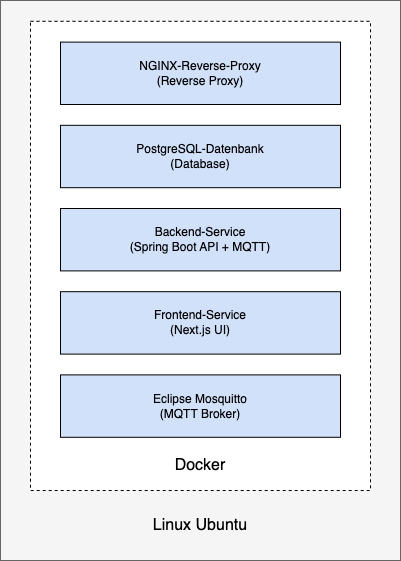
\includegraphics[width=0.3\textwidth]{../figures/deployment-system.drawio.png}
          \caption{Systemübersicht der Linuxumgebung}
          \label{fig:deployment-system}
        \end{figure}

    \subsection{NGINX-Proxykonfiguration}

        Der NGINX-Proxy übernimmt Routing und Zugriffskontrolle. Alle Anfragen werden per http/https direkt auf den Proxy gemacht.
        Dieser aggregiert dann automatisch zum gewünschten Endpunkte. Das Mapping der Endpunkte sieht wie folgt aus:

        \begin{itemize}
            \item \texttt{/v1/}, \texttt{/apikey/}, \texttt{/auth/} $\rightarrow$ Weiterleitung an das Backend.
            \item \texttt{/companion/} $\rightarrow$ Weiterleitung an das Backend mit speziellen CORS-Headern für API-Token Authentifizierung.
            \item \texttt{/} (Root) $\rightarrow$ Weiterleitung an das Frontend.
        \end{itemize}

    \subsection{Docker-Compose-Struktur}

    Die Infrastruktur ist in zwei \texttt{docker-compose.yml}-Dateien organisiert:

    \begin{itemize}
        \item \textbf{Backend-Stack}: NGINX, PostgreSQL, Backend-Service, Mosquitto-Broker.
        \item \textbf{Frontend-Stack}: Separater Container, über das gemeinsame Netzwerk \texttt{yappi\_network} mit dem Backend verbunden.
    \end{itemize}

    \subsection{MQTT-Broker-Konfiguration}

    Eclipse Mosquitto ist ein leichtgewichtiger MQTT-Broker, der im Projekt als zentraler Kommunikationsbroker eingesetzt wird.
    Er sorgt dafür, dass Echtzeit-Benachrichtigungen unabhängig und effizient aggregiert werden können.
    Mosquitto verwaltet den Nachrichtenaustausch zwischen dem Backend, das über MQTT kommuniziert, und der Chrome Extension, die zwingendermassen Websockets verwendet,
    sodass beide Systeme zuverlässig miteinander Daten austauschen können.

    \begin{itemize}
        \item \textbf{TCP-Port 1883} für Backend-Services.
        \item \textbf{WebSocket-Port 9001} für  die Chrome Extension.
    \end{itemize}

    \subsection{Zusammenfassung}

    Durch die Kombination aus GitHub Actions, Docker Compose und NGINX erfolgt der Betrieb der Yappi-Plattform weitgehend automatisiert.
    Codeänderungen werden unmittelbar getestet, gebaut und auf dem SwitchEngines-Server ausgerollt. Dies gewährleistet eine kontinuierliche und zuverlässige Auslieferung neuer Versionen.

\xeno{}
\todo{UML Deployment Diagramm}

%--------------------------------------------------------------------------------------------------------------------------------------

\chapter{Evaluation}
\xeno{}

 \section{Usertesting am Hackathon}

 Ein geplanter Usability-Test wird im Rahmen des an der FHNW stattfindenden Hackathons \textit{Energie-Days} durchgeführt.
 Der Hackathon findet am 11. und 12. September 2025 statt und liegt somit zeitlich nach der Abgabe dieser Arbeit.

 Die Veranstaltung bringt Entwicklerinnen und Entwickler mit unterschiedlichem fachlichen Hintergrund zusammen, die in
 kurzer Zeit kollaborativ Projekte umsetzen. Diese Rahmenbedingungen bieten eine geeignete Gelegenheit, Yappi unter
 realistischen Arbeitsbedingungen zu testen.

 Zum Zeitpunkt der Erstellung dieser Arbeit wurde der Test noch nicht durchgeführt. Es besteht jedoch bereits Kontakt mit
 den Organisatoren, um vor Ort entweder:
 \begin{itemize}
     \item Yappi direkt in einem Entwicklerteam einzusetzen, das die Plattform während des Hackathons aktiv nutzt, oder
     \item eine Befragung von Teilnehmenden an einem Informations- und Teststand durchzuführen.
 \end{itemize}

 Die Durchführung dieses Tests wird es ermöglichen, praxisnahe Rückmeldungen zur Benutzerfreundlichkeit, Funktionalität
 und Integration von Yappi in den Arbeitsfluss zu erhalten. Zusätzlich bieten dieser Test die möglichkeit testdaten zu
 sammeln um weitere erkentnisse zwischen den gesammelten Daten und der Zufriedenheit schaffen.gesammelten Die dabei
 gewonnenen Erkenntnisse sollen in ein Folgeprojekt (IP6) einfliessen.

\section{Evaluation durch Simulation}

Neben dem Praxistest am Hackathon wurde Yappi in einer kontrollierten Testumgebung evaluiert. Ziel ist es, spezifische
Funktionen ohne Abhängigkeit von realen Projektdaten oder sensiblen Informationen zu überprüfen.

Die Simulation erfolgte in mehreren Schritten:
\begin{enumerate}
    \item Zielgruppen und Nutzerrollen festlegen: Definition typischer Nutzerprofile (Personas) wie Softwareentwickler,
    Scrum Master oder Product Owner, inklusive ihrer Ziele und Anforderungen.
    \item Szenarien entwickeln: Erstellung realistischer Nutzungsszenarien, die zentrale Arbeitsabläufe abbilden.
    \item Testpersonen auswählen: Rekrutierung von Personen mit relevanter Erfahrung, jedoch ohne tiefe
    Beteiligung an der Entwicklung von Yappi, um eine objektive Bewertung zu gewährleisten.
    \item Rollen zuweisen: Verteilung der definierten Personas und Szenarien an die Testpersonen mit der Anweisung,
    die Aufgaben wie in einer realen Arbeitssituation durchzuführen.
    \item Testdurchführung: Schrittweises Durchspielen der Szenarien, begleitet von der Methode des lauten Denkens,
    um Nutzungshürden und Verständnisprobleme zu identifizieren.
    \item Ergebniserfassung: Dokumentation der Beobachtungen in Protokollen, Checklisten und standardisierten
    Fragebögen.
    \item Auswertung und Massnahmen: Analyse der Rückmeldungen, Identifikation wiederkehrender Probleme und Ableitung
    konkreter Optimierungsvorschläge.
\end{enumerate}

Diese Simulation ermöglicht es, Funktionen iterativ zu verbessern, bevor sie in realen Teams eingesetzt werden. Eine
kurze Evaluation vor Projektabschluss stellt sicher, dass die vorgenommenen Anpassungen die identifizierten Probleme adressieren.

    \subsection{Nutzerprofil (Persona)}

    \textbf{Persona:} Softwareentwickler/in

    \textbf{Ziele:}
    \begin{itemize}
        \item Arbeitszufriedenheit einfach erfassen.
        \item Persönliche Trends erkennen.
    \end{itemize}

    \textbf{Anforderungen:}
    \begin{itemize}
        \item Schnelle und intuitive Bedienung.
        \item Minimale Unterbrechung des Arbeitsflusses.
    \end{itemize}

    \subsection{Testszenarien}

    Für die Evaluation von Yappi wurden drei Szenarien definiert, die zentrale Funktionen der Plattform abdecken.
    Die Szenarien wurden für die Simulation entwickelt um die funktionen von Yappi zu Testen.

    \subsubsection{Szenario 1: Erfassung der Zufriedenheit nach einem Code-Commit}
    \textbf{Ziel:} Überprüfung der intuitiven Nutzung und Unterbrechungswirkung der Zufriedenheitserfassung über das IDE-Plugin.

    \textbf{Ablauf:}
    \begin{enumerate}
        \item Die Testperson führt eine Programmieraufgabe in IntelliJ IDEA durch.
        \item Nach dem Commit erscheint automatisch eine Benachrichtigung des Yappi-Plugins.
        \item Die Testperson gibt die aktuelle Zufriedenheit über die Eingabemaske ein.
        \item Rückmeldungen zu Verständlichkeit, Geschwindigkeit und Arbeitsfluss werden dokumentiert.
    \end{enumerate}

    \textbf{Bewertungskriterien:}
    \begin{itemize}
        \item Verständlichkeit und Auffindbarkeit der Funktion
        \item Geschwindigkeit des Erfassungsprozesses
        \item Wahrgenommene Unterbrechung des Arbeitsflusses
    \end{itemize}

    \subsubsection{Szenario 2: API-Key mit der Kalenderintegration verbinden}
    \textbf{Ziel:} Überprüfung, ob die Verbindung zwischen Yappi und dem persönlichen Kalender mittels API-Key einfach
    und verständlich hergestellt werden kann. Dabei soll festgestellt werden, ob Nutzerinnen und Nutzer ohne technische
    Unterstützung den Vorgang erfolgreich durchführen.

    \textbf{Ablauf:}
    \begin{enumerate}
        \item Die Testperson ruft in Yappi den Bereich für des Benutzerprofil auf.
        \item Sie generiert oder kopiert einen bestehenden API-Key.
        \item Der API-Key wird in das dafür vorgesehene Feld in der Browsererweiterung eingefügt.
        \item Yappi benachrichtigt automatisch über Kalenderevents.
        \item Rückmeldungen zu Verständlichkeit, benötigter Zeit und auftretenden Schwierigkeiten werden dokumentiert.
    \end{enumerate}

    \textbf{Bewertungskriterien:}
    \begin{itemize}
        \item Verständlichkeit der Anleitung in Yappi
        \item Einfachheit des Kopier- und Einfügevorgangs des API-Keys
        \item Zuverlässigkeit der Synchronisation der Kalenderdaten
        \item Wahrgenommener Zeitaufwand
    \end{itemize}

    \subsubsection{Szenario 3: Meeting-Erfassung über Kalenderintegration}
    \textbf{Ziel:} Validierung der automatischen Erkennung und zeitnahen Erfassung von Meetingwahrnehmungen.

    \textbf{Ablauf:}
    \begin{enumerate}
        \item Ein Testmeeting wird im Kalender der Testperson eingetragen.
        \item Nach beenden des Meeting erhält die Testperson automatisch eine Erinnerung zur Bewertung.
        \item Die Testperson füllt das Feedbackformular aus.
        \item Feedback zu Auslösezeitpunkt, Relevanz und Eingabeprozess wird dokumentiert.
    \end{enumerate}

    \textbf{Bewertungskriterien:}
    \begin{itemize}
        \item Zuverlässigkeit der Meeting-Erkennung
        \item Angemessenheit des Erinnerungszeitpunkts
        \item Vollständigkeit der abgefragten Informationen
    \end{itemize}


%--------------------------------------------------------------------------------------------------------------------------------------

\section{Beantwortung der Fragestellung}

    Die im Projekt verfolgten Forschungsfragen wurden anhand der definierten Produktziele überprüft. Die Beantwortung
    erfolgt nachfolgend in direktem Bezug zu den formulierten Zielen und den erzielten Ergebnissen.

    \subsection*{Forschungsfrage A}
    \textit{Durch welche Technologien und Schnittstellen kann Yappi erweitert werden, um ein reibungsloses und einfaches
    Erfassen von Zufriedenheitsdaten zu ermöglichen?}

    Dieses Ziel wurde im Rahmen der Entwicklung vollständig adressiert. Die Integration in bestehende Arbeitsumgebungen
    erfolgt über:
    \begin{itemize}
        \item ein \textbf{IntelliJ-IDEA-Plugin} zur direkten Erfassung nach einem Code-Commit (Ziel Z-1),
        \item eine \textbf{Kalenderintegration} über das iCalendar-Format zur automatisierten Erkennung von Meetings (Ziel Z-2),
        \item eine \textbf{Browsererweiterung} zur zeitnahen Erfassung der Meetingwahrnehmung (Ziel Z-2).
    \end{itemize}
    Die automatisierte und kontextbezogene Aufforderung reduziert den manuellen Aufwand und erhöht die Regelmässigkeit
    der Erfassungen. Damit wird das Ziel einer nahtlosen Integration in den Arbeitsprozess erreicht.

    \subsection*{Forschungsfrage B}
    \textit{Wie können Gesundheitsdaten in die Auswertung der Entwicklerzufriedenheit einfliessen?}

    Es wurde eine konzeptionelle und teilweise technische Lösung für die Anbindung an \textbf{Apple HealthKit} entwickelt
    (Ziel Z-3). Dadurch können wissenschaftlich relevante Metriken wie Schlafdauer, Ruheherzfrequenz, Stress (HRV) sowie
    Aktivitätsminuten automatisiert erfasst und mit den Zufriedenheitsdaten verknüpft werden.
    Die Integration schafft die Grundlage für weiterführende Analysen zu möglichen Zusammenhängen zwischen physiologischen
    Faktoren und der subjektiven Arbeitszufriedenheit. Aufgrund zeitlicher Einschränkungen wurde diese Anbindung nicht
    vollständig produktiv umgesetzt, die technische Machbarkeit jedoch validiert.

    \subsection*{Forschungsfrage C}
    \textit{Wie kann Yappi Teams und Entwickler dabei unterstützen, aus den erfassten Zufriedenheitsdaten
    Handlungsempfehlungen abzuleiten?}

    Die Entwicklung einer intelligenten Empfehlungskomponente, \textbf{Yappi Coach}, wurde konzeptionell ausgearbeitet
    (Ziel Z-4).
    Das Konzept sieht vor, Zufriedenheitsdaten, Arbeitskontext und Gesundheitsmetriken zu kombinieren, um datenbasierte
    und individuell zugeschnittene Handlungsempfehlungen zu generieren. Eine technische Implementierung erfolgte in diesem
    Projekt nicht, da sie den Rahmen der Arbeit überschreiten würde. Das Konzept bildet jedoch eine belastbare Grundlage
    für ein Folgeprojekt.

    \subsection*{Zusammenfassung}
    Die Ziele Z-1 bis Z-3 wurden in diesem Projekt vollständig oder prototypisch umgesetzt, womit die Forschungsfragen
    A und B beantwortet werden können. Die Forschungsfrage C wurde konzeptionell beantwortet, eine praktische Umsetzung
    ist als nächster Entwicklungsschritt vorgesehen. Insgesamt trägt die Arbeit zur Verbesserung der kontinuierlichen,
    kontextbezogenen und nutzerfreundlichen Erfassung von Entwicklerzufriedenheit bei.


%--------------------------------------------------------------------------------------------------------------------------------------

\chapter{Diskussion}
\section{Reflexion}
\todo{}

\printbibliography

\end{document}
